\newpage
\chapter{CONSTRUCCIÓN DEL SISTEMA DE INFORMACIÓN}
	\vspace{2cm}	
	\begin{center}
	{\Large \textbf{FASE DE DESARROLLO} \par}
	\end{center}
	\vspace{5cm}
	
	\begin{center}
	\Huge \textbf{CSI}\par
	\end{center}

\newpage


\section[CSI 1: PREPARACIÓN DEL ENTORNO DE GENERACIÓN Y \\ CONSTRUCCIÓN]{CSI 1: PREPARACIÓN DEL ENTORNO DE GENERACIÓN Y CONSTRUCCIÓN}

\subsection{Estándares y normas seguidos}
\subsubsection{Angular Style Guide}
La guía de estilos de Angular\cite{AngularSG} es un conjunto de recomendaciones sobre la sintaxis, estructura y convenciones de código en proyectos de Angular.
\subsubsection{HTML5}
HTML5 es la versión más reciente y la actualmente usada de HTML, y está estandarizada por el W3C (World Wide Web Consortium).
\subsubsection{CSS}
Hojas de estilos estandarizadas por el W3C.
\subsubsection{PHP Code Style Guide}
La guía de estilos de PHP\cite{PhpSG} contiene normas de código y buenas prácticas.

\subsection{Lenguajes de programación}
\subsubsection{TypeScript}
TypeScript es un lenguaje de programación de código abierto desarrollado por Microsoft. Extiende JavaScript añadiendo la definición de tipos estáticos.
\subsubsection{HTML}
HTML (HyperText Markup Language) es un lenguaje de marcado utilizado en la elaboración de páginas web.
\subsubsection{CSS}
CSS (Cascading Style Sheets) es un lenguaje de diseño gráfico que permite modificar la presentación de los elementos definidos en los documentos HTML.
\subsubsection{PHP}
PHP es un lenguaje de programación utilizado en el desarrollo web que es procesado en el lado del servidor.
\subsubsection{SQL}
SQL (Structured Query Language) es un lenguaje de consultas utilizado para leer, insertar, actualizar o eliminar datos de la base de datos relacional utilizada. 
\subsection{Herramientas y programas usados para el desarrollo}
\subsubsection{Visual Studio Code}
Visual Studio Code es un editor de código fuente desarrollado por Microsoft, gratuito y de código abierto. Tiene soporte integrado para TypeScript y Node.js, extensiones para otros lenguajes como PHP. También cuenta con soporte para depuración, control integrado de Git e \textit{IntelliSense}, una función de autocompletado de código\cite{VSCode}.
\begin{figure}[H]
	\centering
	
\includegraphics[scale=0.05]{vscode}
	\caption{Logo de Visual Studio Code}
\end{figure}
\subsubsection{XAMPP}
XAMPP es una distribución de Apache gratuita que contiene MariaDB, PHP y Perl\cite{Xampp}. Fue usado inicialmente para trabajar con la base de datos y los PHP necesarios, pero una vez configurado el servidor Ubuntu 20.04 dejó de ser necesario.
\begin{figure}[H]
	\centering
	
\includegraphics[scale=0.3]{xampp}
	\caption{Logo de XAMPP}
\end{figure}
\subsubsection{MobaXTerm}
MobaXTerm permite trabajar con herramientas de red remotas, como SSH, utilizando una terminal Unix desde Windows. Se ha usado para configurar la máquina Ubuntu 20.04 que aloja el servidor MySQL con la base de datos del sistema, y el servidor Apache con las aplicaciones y los archivos PHP desarrollados.
\begin{figure}[H]
	\centering
	\includegraphics[scale=0.5]{MobaXTerm}
	\caption{Logo de MobaXTerm}
\end{figure}

\subsubsection{Git}
Git es un software de control de versiones gratuito y de código abierto, diseñado para gestionar los cambios de un repositorio\cite{Git}.
\begin{figure}[H]
	\centering
	
\includegraphics[scale=0.2]{git}
	\caption{Logo de Git}
\end{figure}

\newpage
\section[CSI 2: GENERACIÓN DEL CÓDIGO DE LOS COMPONENTES Y \\ PROCEDIMIENTOS]{CSI 2: GENERACIÓN DEL CÓDIGO DE LOS COMPONENTES Y PROCEDIMIENTOS}
Una vez desarrolladas las aplicaciones del museo y la administración, se han documentado las clases de ambos proyectos. Esta documentación se ha generado utilizando \textit{Compodoc}\cite{compodoc}, una herramienta similar a la conocida JavaDoc para Angular. Debido a la extensión de la documentación los dos proyectos, se adjunta como archivos externos, como se indica más adelante en el Contenido entregado en los anexos (sección \ref{sec:contenido_anexos}).


\newpage
\section{CSI 3: EJECUCIÓN DE LAS PRUEBAS UNITARIAS}
A continuación se muestran los listados de las pruebas unitarias realizadas con KarmaJS y JasmineJS, así como los porcentajes de cobertura de código.\par
\begin{figure}[H]
\centering
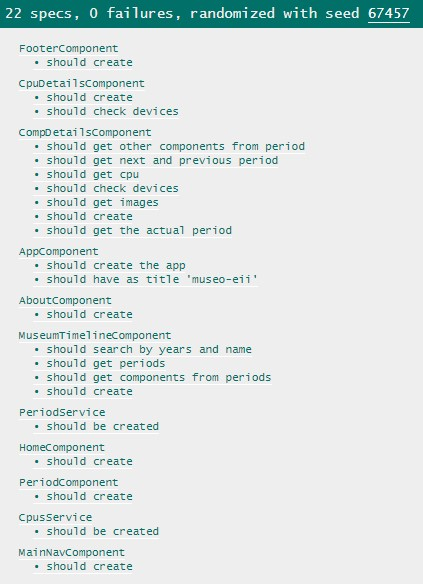
\includegraphics[scale=0.8]{unit-tests-museo}
\caption{Ejecución de las pruebas unitarias del museo}
\end{figure}
\begin{figure}[H]
\centering
\centerline{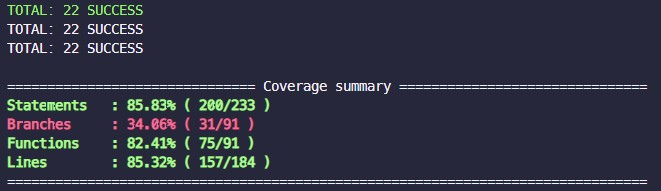
\includegraphics[scale=0.8]{coverage-museo}}
\caption{Cobertura de código de las pruebas unitarias del museo}
\end{figure}
En las pruebas unitarias de la administración hubo algunos fallos, como se puede ver a continuación.\par
Aquí se puede observar que al probar a eliminar un periodo existente, este no se borraba. Tras revisar el código, caí en la cuenta de que solo había hecho mocks de los servicios HTTP que usa la aplicación, y debía hacerlo también para el diálogo de confirmación ya que si no, el método de eliminar no se terminaría de ejecutar. Una vez añadido este mock la prueba pasó sin fallos.
\begin{figure}[H]
\centering
\centerline{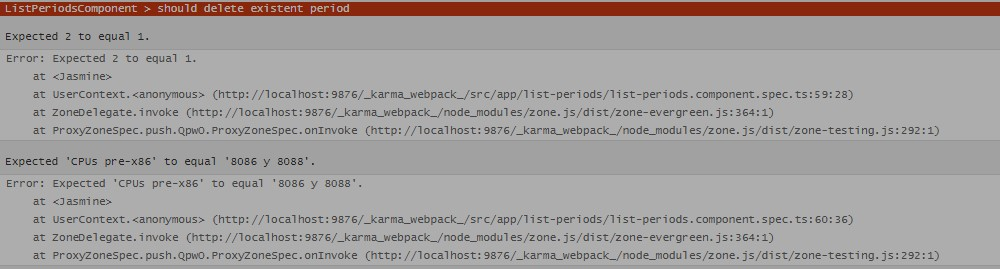
\includegraphics[scale=0.7]{error-test-admin}}
\caption{Error en la prueba de eliminar un periodo existente}
\end{figure}
\begin{figure}[H]
\centering
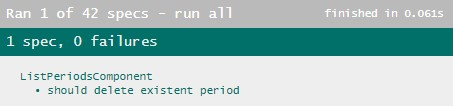
\includegraphics[scale=1]{error-test-admin-fix}
\caption{Eliminar un periodo existente tras la corrección de la prueba}
\end{figure}
\begin{figure}[H]
\hspace{-10mm}
\begin{subfigure}[b]{0.6\textwidth}
\centering
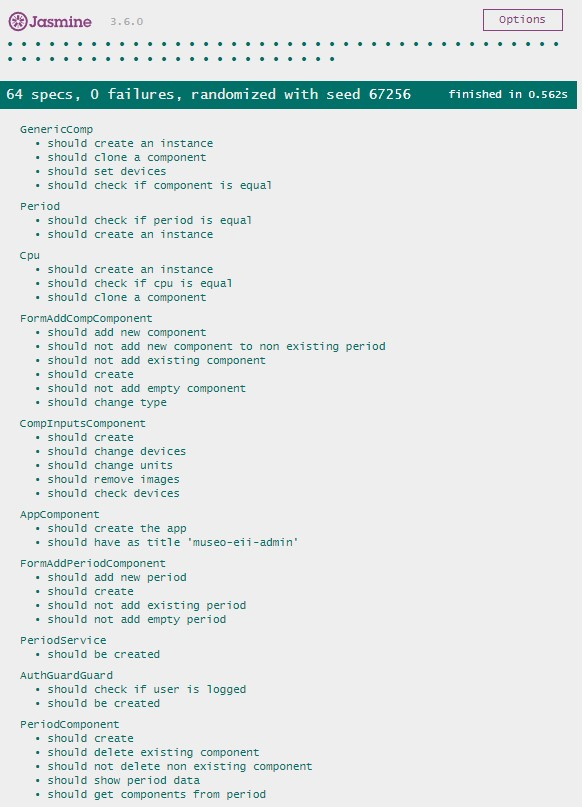
\includegraphics[scale=0.8]{unit-tests-admin}
\end{subfigure}
\begin{subfigure}[b]{0.4\textwidth}
\centering
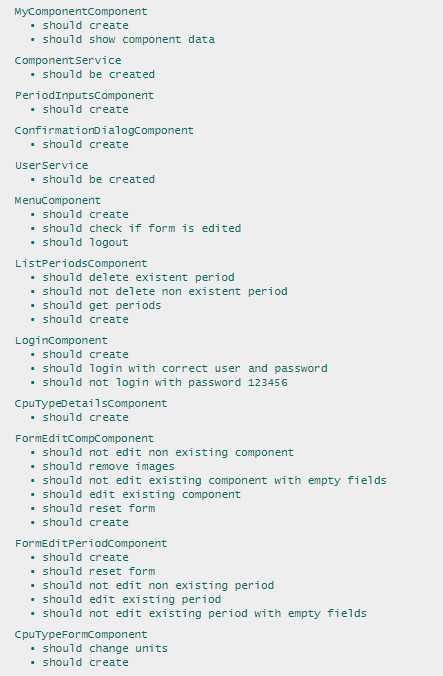
\includegraphics[scale=0.8]{unit-tests-admin-2}
\end{subfigure}
\caption{Ejecución de las pruebas unitarias de la administración}
\end{figure}
\begin{figure}[H]
\centering
\centerline{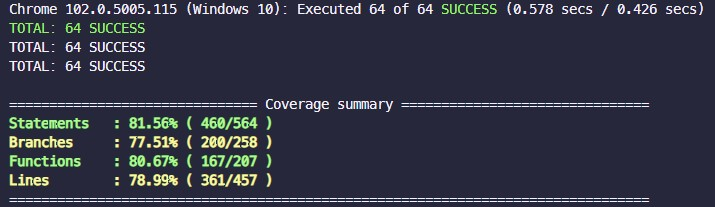
\includegraphics[scale=0.8]{coverage-admin}}
\caption{Cobertura de código de las pruebas unitarias de la administración}
\end{figure}

\newpage
\section{CSI 4: EJECUCIÓN DE LAS PRUEBAS DE INTEGRACIÓN}
Como se mencionó en la especificación del plan de pruebas (sección \ref{sec:pruebas-sistema}) estas pruebas se realizaron de forma manual sobre la aplicación.
\begin{table}[H]
%\vspace{-4mm}
  \centering
  \caption{Ejecución de pruebas: Consultar periodos (museo)}
    \begin{tabular}{p{9em}p{22em}p{5em}}
    \toprule
    \rowcolor[rgb]{ .851,  .886,  .953} \multicolumn{3}{p{36em}}{\textbf{Consultar periodos (museo)}} \\ \midrule
    \rowcolor[rgb]{ .949,  .949,  .949} \textbf{Prueba} & \textbf{Resultado esperado} & \textbf{¿Superado?} \\ \midrule
    \textbf{Obtener periodos existentes} & El sistema devolverá una lista de todos los periodos existentes. & Sí \\ \midrule
    \textbf{Obtener periodo por nombre} & El sistema devolverá una lista de los periodos cuyo nombre contenga el texto introducido. & Sí \\ \midrule
    \textbf{Obtener periodo por años} & El sistema devolverá una lista de los periodos cuyos años coincidan con los introducidos. & Sí \\ \bottomrule
    \end{tabular}%
\end{table}%
\begin{table}[H]
\vspace{-4mm}
  \centering
  \caption{Ejecución de pruebas: Consultar componentes (museo)}
    \begin{tabular}{p{11em}p{20em}p{5em}}
    \toprule
    \rowcolor[rgb]{ .851,  .886,  .953} \multicolumn{3}{p{36em}}{\textbf{Consultar componentes (museo)}} \\ \midrule
    \rowcolor[rgb]{ .949,  .949,  .949} \textbf{Prueba} & \textbf{Resultado esperado} & \textbf{¿Superado?} \\ \midrule
    \textbf{Obtener componentes de un periodo} & El sistema devolverá una lista de todos los componentes pertenecientes al periodo. & Sí \\ \bottomrule
    \end{tabular}%
\end{table}%
\begin{table}[H]
\vspace{-4mm}
  \centering
  \caption{Ejecución de pruebas: Iniciar sesión}
    \begin{tabular}{p{9em}p{22em}p{5em}}
    \toprule
    \rowcolor[rgb]{ .851,  .886,  .953} \multicolumn{3}{p{36em}}{\textbf{Iniciar sesión}} \\ \midrule
    \rowcolor[rgb]{ .949,  .949,  .949} \textbf{Prueba} & \textbf{Resultado esperado} & \textbf{¿Superado?} \\ \midrule
    \textbf{Iniciar sesión con datos válidos } & El sistema permitirá el acceso a la página de administración.  & Sí \\ \midrule
    \textbf{Iniciar sesión con datos incorrectos} & El sistema no permitirá el acceso y se mostrará un error.  & Sí \\ \bottomrule
    \end{tabular}%
\end{table}%
\begin{table}[H]
\vspace{-4mm}
  \centering
  \caption{Ejecución de pruebas: Consultar periodos (administración)}
    \begin{tabular}{p{9em}p{22em}p{5em}}
    \toprule
    \rowcolor[rgb]{ .851,  .886,  .953} \multicolumn{3}{p{36em}}{\textbf{Consultar periodos (administración)}} \\ \midrule
    \rowcolor[rgb]{ .949,  .949,  .949} \textbf{Prueba} & \textbf{Resultado esperado} & \textbf{¿Superado?} \\ \midrule
    \textbf{Obtener periodos existentes} & El sistema devolverá una lista de todos los periodos existentes.  & Sí \\ \bottomrule
    \end{tabular}%
\end{table}%
\begin{table}[H]
\vspace{-4mm}
  \centering
  \caption{Ejecución de pruebas: Añadir periodo}
    \begin{tabular}{p{8em}p{23em}p{5em}}
    \toprule
    \rowcolor[rgb]{ .851,  .886,  .953} \multicolumn{3}{p{36em}}{\textbf{Añadir periodo}} \\ \midrule
    \rowcolor[rgb]{ .949,  .949,  .949} \textbf{Prueba} & \textbf{Resultado esperado} & \textbf{¿Superado?} \\ \midrule
    \textbf{Añadir nuevo periodo (periodo 2)} & El sistema tendrá un periodo más.  & Sí \\ \midrule
    \textbf{Añadir periodo que ya existe (periodo 1)} & El sistema no añadirá el periodo y responderá con un error.  & Sí  \\ \midrule
    \textbf{Añadir periodo con campos vacíos} & El sistema no añadirá el periodo y responderá con un error.  & Sí \\ \bottomrule
    \end{tabular}%
\end{table}%
\begin{table}[H]
\vspace{-4mm}
  \centering
  \caption{Ejecución de pruebas: Modificar periodo}
    \begin{tabular}{p{10em}p{21em}p{5em}}
    \toprule
    \rowcolor[rgb]{ .851,  .886,  .953} \multicolumn{3}{p{36em}}{\textbf{Modificar periodo}} \\ \midrule
    \rowcolor[rgb]{ .949,  .949,  .949} \textbf{Prueba} & \textbf{Resultado esperado} & \textbf{¿Superado?} \\ \midrule
    \textbf{Modificar periodo existente (periodo 1)} & El sistema actualizará los datos del periodo. & Sí  \\ \midrule
    \textbf{Modificar un periodo que no existe (periodo 25)} & El sistema responderá con un error.  & Sí \\ \midrule
    \textbf{Modificar periodo dejando campos vacíos} & El sistema no actualizará el periodo y responderá con un error.  & Sí \\ \bottomrule
    \end{tabular}%
\end{table}%
\begin{table}[H]
\vspace{-4mm}
  \centering
  \caption{Ejecución de pruebas: Eliminar periodo}
    \begin{tabular}{p{11em}p{20em}p{5em}}
    \toprule
    \rowcolor[rgb]{ .851,  .886,  .953} \multicolumn{3}{p{36em}}{\textbf{Eliminar periodo}} \\ \midrule
    \rowcolor[rgb]{ .949,  .949,  .949} \textbf{Prueba} & \textbf{Resultado esperado} & \textbf{¿Superado?} \\ \midrule
    \textbf{Eliminar un periodo existente (periodo 1)} & El sistema tendrá un periodo menos.  & Sí \\ \midrule
    \textbf{Eliminar un periodo que no existe (periodo 25)} & El sistema responderá con un error.  & Sí \\ \bottomrule
    \end{tabular}%
\end{table}%
\begin{table}[H]
\vspace{-4mm}
  \centering
  \caption{Ejecución de pruebas: Consultar componentes (administración)}
    \begin{tabular}{p{11em}p{20em}p{5em}}
    \toprule
    \rowcolor[rgb]{ .851,  .886,  .953} \multicolumn{3}{p{36em}}{\textbf{Consultar componentes (administración)}} \\ \midrule
    \rowcolor[rgb]{ .949,  .949,  .949} \textbf{Prueba} & \textbf{Resultado esperado} & \textbf{¿Superado?} \\ \midrule
    \textbf{Obtener componentes de un periodo} & El sistema devolverá una lista de todos los componentes pertenecientes al periodo.  & Sí \\ \bottomrule
    \end{tabular}%
\end{table}%
\begin{table}[H]
\vspace{-4mm}
  \centering
  \caption{Ejecución de pruebas: Añadir componente}
    \begin{tabular}{p{13em}p{18em}p{5em}}
    \toprule
    \rowcolor[rgb]{ .851,  .886,  .953} \multicolumn{3}{p{36em}}{\textbf{Añadir componente}} \\ \midrule
    \rowcolor[rgb]{ .949,  .949,  .949} \textbf{Prueba} & \textbf{Resultado esperado} & \textbf{¿Superado?} \\ \midrule
    \textbf{Añadir nuevo componente (CPU 2)} & El sistema tendrá un componente más.  & Sí  \\ \midrule
    \textbf{Añadir componente que ya existe (CPU 1)} & El sistema no añadirá el componente y responderá con un error.  & Sí  \\ \midrule
    \textbf{Añadir componente a un periodo que no existe (CPU 3, periodo 25)} & El sistema no añadirá el componente y responderá con un error.  & Sí  \\ \midrule
    \textbf{Añadir componente con campos obligatorios vacíos} & El sistema no añadirá el componente y responderá con un error.  & Sí \\ \bottomrule
    \end{tabular}%
\end{table}%
\begin{table}[H]
\vspace{-4mm}
  \centering
  \caption{Ejecución de pruebas: Modificar componente}
    \begin{tabular}{p{13em}p{18em}p{5em}}
    \toprule
    \rowcolor[rgb]{ .851,  .886,  .953} \multicolumn{3}{p{36em}}{\textbf{Modificar componente}} \\ \midrule
    \rowcolor[rgb]{ .949,  .949,  .949} \textbf{Prueba} & \textbf{Resultado esperado} & \textbf{¿Superado?} \\ \midrule
    \textbf{Modificar componente existente (CPU 1)} & El sistema actualizará los datos del componente.  & Sí \\ \midrule
    \textbf{Modificar un componente que no existe (CPU 30)} & El sistema responderá con un error.  & Sí \\ \midrule
    \textbf{Modificar componente dejando campos obligatorios vacíos} &  El sistema no actualizará el componente y responderá con un error.  & Sí \\ \bottomrule
    \end{tabular}%
\end{table}%
\begin{table}[H]
\vspace{-4mm}
  \centering
  \caption{Ejecución de pruebas: Eliminar componente}
    \begin{tabular}{p{13em}p{18em}p{5em}}
    \toprule
    \rowcolor[rgb]{ .851,  .886,  .953} \multicolumn{3}{p{36em}}{\textbf{Eliminar componente}} \\ \midrule
    \rowcolor[rgb]{ .949,  .949,  .949} \textbf{Prueba} & \textbf{Resultado esperado} & \textbf{¿Superado?} \\ \midrule
    \textbf{Eliminar un componente existente (CPU 1)} & El sistema tendrá un componente menos.  & Sí  \\ \midrule
    \textbf{Eliminar un componente que no existe (CPU 30)} &  El sistema responderá con un error.  & Sí  \\ \bottomrule
    \end{tabular}%
\end{table}%

\newpage
\section{CSI 5: EJECUCIÓN DE LAS PRUEBAS DEL SISTEMA}
\subsection{Prueba de Usabilidad}
Una vez desarrollada la aplicación, podemos pasar la guía de usabilidad desarrollada por Yusef Hassan Montero\cite{Usabilidad}.
\begin{longtable}[H]{p{31em}|p{5em}}
\caption{Checklist de pruebas de Usabilidad}
\\ \hline  \\[-1em]
\cellcolor[rgb]{.949,  .949,  .949} \textbf{Criterios} & \cellcolor[rgb]{.949,  .949,  .949}\textbf{¿Cumplido?} \\ \hline  \\[-1em]
\multicolumn{2}{p{36em}}{\cellcolor[rgb]{ .851,  .886,  .953} \textbf{Generales}} \\ \hline \\[-1em]
\textbf{¿Cuáles son los objetivos del sitio web? ¿Son concretos y bien definidos? ¿Los contenidos y servicios que ofrece se corresponden con esos objetivos?} & Sí \\ \hline \\[-1em]
\textbf{¿Tiene una URL correcta, clara y fácil de recordar? ¿Y las URL de sus páginas internas? ¿Son claras y permanentes?} & Sí \\ \hline \\[-1em]
\textbf{¿Muestra de forma precisa y completa qué contenidos o servicios ofrece realmente el sitio web?} El diseño de la página de inicio debe ser diferente al resto de páginas y cumplir la función de 'escaparate' del sitio. & Sí \\ \hline \\[-1em]
\textbf{¿La estructura general del sitio web está orientada al usuario?} Los sitios web deben estructurarse pensando en el usuario, sus objetivos y necesidades. La estructura interna de la empresa u organización, cómo funciona o se organiza no interesan al usuario. & Sí \\ \hline \\[-1em]
\textbf{¿El look \& feel general se corresponde con los objetivos, características, contenidos y servicios del sitio web?} Ciertas combinaciones de colores ofrecen imágenes más o menos formales, serias o profesionales. & Sí \\ \hline \\[-1em]
\textbf{¿Es coherente el diseño general del sitio web?} Se debe mantener una coherencia y uniformidad en las estructuras y colores de todas las páginas. Esto sirve para que el usuario no se desoriente en su navegación. & Sí \\ \hline \\[-1em]
\textbf{¿Es reconocible el diseño general del sitio web?} Cuánto más se parezca el sitio web al resto de sitios web, más fácil será de usar. & Sí \\ \hline \\[-1em]
\textbf{¿El sitio web se actualiza periódicamente? ¿Indica cuándo se actualiza?} Las fechas que se muestren en la página deben corresponderse con actualizaciones, noticias, eventos...no con la fecha del sistema del usuario. & - \\ \hline \\[-1em]
\multicolumn{2}{p{36em}}{\cellcolor[rgb]{ .851,  .886,  .953} \textbf{Identidad e información}} \\ \hline \\[-1em]
\textbf{¿Se muestra claramente la identidad de la empresa-sitio a través de todas las páginas?} & Sí \\ \hline \\[-1em]
El Logotipo, \textbf{¿es significativo, identificable y suficientemente visible?} & Sí \\ \hline \\[-1em]
El eslogan o tagline, \textbf{¿expresa realmente qué es la empresa y qué servicios ofrece?} & - \\ \hline \\[-1em]
\textbf{¿Se ofrece algún enlace con información sobre la empresa, sitio web, 'webmaster’...? } & Sí \\ \hline \\[-1em]
\textbf{¿Se proporciona mecanismos para ponerse en contacto con la empresa?} (email, teléfono, dirección postal, fax...) & - \\ \hline \\[-1em]
\textbf{¿Se proporciona información sobre la protección de datos de carácter personal de los clientes o los derechos de autor de los contenidos del sitio web?} & - \\ \hline \\[-1em]
En artículos, noticias, informes... \textbf{¿Se muestra claramente información sobre el autor, fuentes y fechas de creación y revisión del documento? } & - \\ \hline \\[-1em]
\multicolumn{2}{p{36em}}{\cellcolor[rgb]{ .851,  .886,  .953} \textbf{Lenguaje y redacción}} \\ \hline \\[-1em]
\textbf{¿El sitio web habla el mismo lenguaje que sus usuarios?} Se debe evitar usar un lenguaje corporativista. Así mismo, hay que prestarle especial atención al idioma, y ofrecer versiones del sitio en diferentes idiomas cuando sea necesario. & Sí \\ \hline \\[-1em]
\textbf{¿Emplea un lenguaje claro y conciso?} & Sí \\ \hline \\[-1em]
\textbf{¿Es amigable, familiar y cercano?} Es decir, lo contrario a utilizar un lenguaje constantemente imperativo, mensajes crípticos, o tratar con "desprecio" al usuario. & Sí \\ \hline \\[-1em]
\textbf{¿1 párrafo = 1 idea?} Cada párrafo es un objeto informativo. Trasmita ideas, mensajes...Se deben evitar párrafos vacíos o varios mensajes en un mismo párrafo. & Sí \\ \hline \\[-1em]
\multicolumn{2}{p{36em}}{\cellcolor[rgb]{ .851,  .886,  .953} \textbf{Rotulado}} \\ \hline \\[-1em]
Los rótulos, \textbf{¿son significativos?} Ejemplo: evitar rótulos del tipo "haga clic aquí". & Sí \\ \hline \\[-1em]
\textbf{¿Usa rótulos estándar?} Siempre que exista un "estándar" comúnmente aceptado para el caso concreto, como "Mapa del Sitio" o "Acerca de...". & Sí \\ \hline \\[-1em]
\textbf{¿Usa un único sistema de organización, bien definido y claro?} No se deben mezclar diferentes. Los sistemas de organización son: alfabético, geográfico, cronológico, temático, orientado a tareas, orientado al público y orientado a metáforas. & Sí \\ \hline \\[-1em]
\textbf{¿Utiliza un sistema de rotulado controlado y preciso?} Por ejemplo, si un enlace tiene el rótulo "Quiénes somos", no puede dirigir a una página cuyo encabezamiento sea "Acerca de" & Sí \\ \hline \\[-1em]
El título de las páginas, \textbf{¿Es correcto? ¿Ha sido planificado?} Relacionado con la capacidad para poder buscar y encontrar el sitio web. & Sí \\ \hline \\[-1em]
\multicolumn{2}{p{36em}}{\cellcolor[rgb]{ .851,  .886,  .953} \textbf{Estructura y navegación}} \\ \hline \\[-1em]
La estructura de organización y navegación, \textbf{¿Es la más adecuada?} Hay varios tipos de estructuras: jerárquicas, hipertextual, facetada... & Sí \\ \hline \\[-1em]
En el caso de estructura jerárquica, \textbf{¿Mantiene un equilibrio entre Profundidad y Anchura?} & - \\ \hline \\[-1em]
En el caso de ser puramente hipertextual, \textbf{¿Están todos los clústeres de nodos comunicados?} Aquí se mide la distancia entre nodos. & Sí \\ \hline \\[-1em]
\textbf{¿Los enlaces son fácilmente reconocibles como tales? ¿Su caracterización indica su estado (visitados, activos...)?} Los enlaces no sólo deben reconocerse como tales, sino que su caracterización debe indicar su estado, y ser reconocidos como una unidad  & No \\ \hline \\[-1em]
En menús de navegación, \textbf{¿Se ha controlado el número de elementos y de términos por elemento para no producir sobrecarga memorística?} No se deben superar los 7±2 elementos, ni los 2 o, como mucho, 3 términos por elemento. & Sí \\ \hline \\[-1em]
\textbf{¿Es predecible la respuesta del sistema antes de hacer clic sobre el enlace?} Relacionado con el nivel de significación del rótulo del enlace, aunque también con: el uso de globos de texto, información contextual, la barra de estado del navegador... & Sí \\ \hline \\[-1em]
\textbf{¿Se ha controlado que no haya enlaces que no llevan a ningún sitio?} Enlaces que no llevan a ningún sitio: Los enlaces rotos, y los que enlazan con la misma página que se está visualizando (por ejemplo, enlaces a la "home" desde la misma página de inicio) & Sí \\ \hline \\[-1em]
\textbf{¿Existen elementos de navegación que orienten al usuario acerca de dónde está y cómo deshacer su navegación?} ...como breadcrumbs, enlaces a la página de inicio...recuerde que el logo también es recomendable que enlace con la página de inicio. & Sí \\ \hline \\[-1em]
Las imágenes enlace, \textbf{¿se reconocen como clicables? ¿Incluyen un atributo 'title' describiendo la página de destino?} En este sentido, también hay que cuidar que no haya imágenes que parezcan enlaces y en realidad no lo sean. & No \\ \hline \\[-1em]
\textbf{¿Se ha evitado la redundancia de enlaces?} & Sí \\ \hline \\[-1em]
\textbf{¿Se ha controlado que no haya páginas "huérfanas"?} Páginas huérfanas: que, aun siendo enlazadas desde otras páginas, éstas no enlacen con ninguna.  & Sí \\ \hline \\[-1em]
\multicolumn{2}{p{36em}}{\cellcolor[rgb]{ .851,  .886,  .953} \textbf{Layout de la página}} \\ \hline \\[-1em]
\textbf{¿Se aprovechan las zonas de alta jerarquía informativa de la página para contenidos de mayor relevancia?} (como por ejemplo la zona central)  & Sí \\ \hline \\[-1em]
\textbf{¿Se ha evitado la sobrecarga informativa?} Esto se consigue haciendo un uso correcto de colores, efectos tipográficos y agrupaciones para discriminar información. Los grupos diferentes de objetos informativos de una página deben ser 7±2.  & Sí \\ \hline \\[-1em]
\textbf{¿Es una interfaz limpia, sin ruido visual?} & Sí \\ \hline \\[-1em]
\textbf{¿Existen zonas en "blanco" entre los objetos informativos de la página para poder descansar la vista?} & Sí \\ \hline \\[-1em]
\textbf{¿Se hace un uso correcto del espacio visual de la página?} Es decir, que no se desaproveche demasiado espacio con elementos de decoración, o grandes zonas en "blanco", y que no se adjudique demasiado espacio a elementos de menor importancia.  & Sí \\ \hline \\[-1em]
\textbf{¿Se utiliza correctamente la jerarquía visual para expresar las relaciones del tipo \"parte de\" entre los elementos de la página?} (La jerarquía visual se utiliza para orientar al usuario) & Sí \\ \hline \\[-1em]
\textbf{¿Se ha controlado la longitud de página?} Se debe evitar en la medida de lo posible el scrolling. Si la página es muy extensa, se debe fraccionar.  & No \\ \hline \\[-1em]
\multicolumn{2}{p{36em}}{\cellcolor[rgb]{ .851,  .886,  .953} \textbf{Elementos multimedia}} \\ \hline \\[-1em]
\textbf{¿Las fotografías están bien recortadas? ¿Son comprensibles? ¿Se ha cuidado su resolución? } & Sí \\ \hline \\[-1em]
\textbf{¿Las metáforas visuales son reconocibles y comprensibles por cualquier usuario?} (prestar especial atención a usuarios de otros países y culturas)  & - \\ \hline \\[-1em]
\textbf{¿El uso de imágenes o animaciones proporciona algún tipo de valor añadido? } & Sí \\ \hline \\[-1em]
\textbf{¿Se ha evitado el uso de animaciones cíclicas?} & Sí \\ \hline \\[-1em]
\multicolumn{2}{p{36em}}{\cellcolor[rgb]{ .851,  .886,  .953} \textbf{Accesibilidad}} \\ \hline \\[-1em]
\textbf{¿El tamaño de fuente se ha definido de forma relativa, o por lo menos, la fuente es lo suficientemente grande como para no dificultar la legibilidad del texto? } & Sí \\ \hline \\[-1em]
\textbf{¿El tipo de fuente, efectos tipográficos, ancho de línea y alineación empleadas facilitan la lectura?} & Sí \\ \hline \\[-1em]
\textbf{¿Existe un alto contraste entre el color de fuente y el fondo?} & Sí \\ \hline \\[-1em]
\textbf{¿Incluyen las imágenes atributos 'alt' que describan su contenido? } & Sí \\ \hline \\[-1em]
\textbf{¿Es compatible el sitio web con los diferentes navegadores? ¿Se visualiza correctamente con diferentes resoluciones de pantalla?} Se debe prestar atención a: JScript, CSS, tablas, fuentes...  & Sí \\ \hline \\[-1em]
\textbf{¿Puede el usuario disfrutar de todos los contenidos del sitio web sin necesidad de tener que descargar e instalar plugins adicionales?} & Sí \\ \hline \\[-1em]
\textbf{¿Se ha controlado el peso de la página?} Se deben optimizar las imágenes, controlar el tamaño del código JScript...  & No \\ \hline \\[-1em]
\textbf{¿Se puede imprimir la página sin problemas?} Leer en pantalla es molesto, por lo que muchos usuarios preferirán imprimir las páginas para leerlas. Se debe asegurar que se puede imprimir la página (no salen partes cortadas), y que el resultado es legible.  & Sí \\ \hline \\[-1em]
\multicolumn{2}{p{36em}}{\cellcolor[rgb]{ .851,  .886,  .953} \textbf{Control y retroalimentación}} \\ \hline \\[-1em]
\textbf{¿Tiene el usuario todo el control sobre el interfaz?} Se debe evitar el uso de ventanas pop-up, ventanas que se abren a pantalla completa, banners intrusivos...  & Sí \\ \hline \\[-1em]
\textbf{¿Se informa constantemente al usuario acerca de lo que está pasando?} Si el usuario tiene que esperar hasta que se termine una operación, se debe mostrar un mensaje indicándoselo y que debe esperar, con el tiempo de espera estimado o una barra de progreso.  & - \\ \hline \\[-1em]
\textbf{¿Se informa al usuario de lo que ha pasado?} Por ejemplo, cuando un usuario valora un artículo o responde a una encuesta, se le debe informar de que su voto ha sido procesado correctamente. & Sí \\ \hline \\[-1em]
Cuando se produce un error, \textbf{¿se informa de forma clara y no alarmista al usuario de lo ocurrido y de cómo solucionar el problema?} Siempre es mejor intentar evitar que se produzcan errores a tener que informar al usuario del error.  & Sí \\ \hline \\[-1em]
\textbf{¿Posee el usuario libertad para actuar?} NO restringir la libertad del usuario: Uso de animaciones que no pueden ser "saltadas", páginas en las que desaparecen los botones de navegación, no impida al usuario poder usar el botón derecho de su ratón... & Sí \\ \hline \\[-1em]
\textbf{¿Se ha controlado el tiempo de respuesta?} Esto tiene que ver con el peso de cada página (accesibilidad) y tiene relación con el tiempo que tarda el servidor en finalizar una tarea y responder. El tiempo máximo que esperará un usuario son 10 segundos  & Sí \\ \hline \\[-1em]
\multicolumn{2}{p{36em}}{\cellcolor[rgb]{ .851,  .886,  .953} \textbf{Aclaraciones}} \\ \hline \\[-1em]
\textbf{¿Se ha evaluado adecuadamente la orientación del usuario?} (Donde estoy, como volver, que he visitado, que va a pasar) & Sí \\ \hline \\[-1em]
\textbf{¿Se ha usado correctamente la publicidad?} & - \\ \hline
\end{longtable}


A continuación, se mostrarán las respuestas de los usuarios a los cuestionarios diseñados anteriormente (sección \ref{sec:cuestionario-usabilidad}). Las pruebas han sido realizadas con tres usuarios para el museo y con el tutor del trabajo para la administración.
\paragraph*{Usuario 1}
\begin{table}[H]
\centering
\caption{Cuestionario de carácter general (Usuario 1)}
\begin{tabular}{p{36em}}
\toprule
\rowcolor[rgb]{ .949,  .949,  .949} \textbf{¿Usa un ordenador frecuentemente?} \\ \midrule
\vspace{-4mm}
\begin{enumerate}
\item \colorbox{blue!30}{Todos los días}
\item Varias veces a la semana
\item Ocasionalmente
\item Nunca
\end{enumerate} \\ \midrule
\rowcolor[rgb]{ .949,  .949,  .949} \textbf{¿Qué tipo de actividades realiza con el ordenador?} \\ \midrule
\vspace{-4mm}
\begin{enumerate}
\item Es parte de mi trabajo o profesión
\item \colorbox{blue!30}{Lo uso básicamente para ocio}
\item Solo empleo aplicaciones estilo Office
\item Únicamente leo el correo y navego ocasionalmente
\end{enumerate} \\ \midrule
\rowcolor[rgb]{ .949,  .949,  .949} \textbf{¿Qué busca Vd. principalmente en una aplicación web?} \\ \midrule
\vspace{-4mm}
\begin{enumerate}
\item \colorbox{blue!30}{Que sea fácil de navegar}
\item Que sea intuitiva
\item Que sea rápida
\item Que tenga todas las funciones necesarias
\end{enumerate} \\ \bottomrule
\end{tabular}
\end{table}

\begin{table}[H]
\centering
\caption{Cuestionario sobre la aplicación (Usuario 1)}
\begin{tabular}{p{15em}|p{4em}|p{7.5em}|p{7.5em}|p{3em}}
\toprule
\rowcolor[rgb]{.949,  .949,  .949} \textbf{Facilidad de uso} & \textbf{Siempre} & \textbf{Frecuentemente} & \textbf{Ocasionalmente} & \textbf{Nunca} \\ \midrule
\textit{¿Sabe dónde está dentro de la aplicación?} & X& & & \\ \midrule
\textit{¿Necesita ayuda para utilizar la aplicación?} & & & &X \\ \midrule
\textit{¿Le resulta sencillo el uso de la aplicación?} &X & & & \\ \midrule
\textit{¿Identifica fácilmente la información que se le presenta?} & X& & & \\ \midrule
\rowcolor[rgb]{.949,  .949,  .949} \textbf{Funcionalidad} & \textbf{Siempre} & \textbf{Frecuentemente} & \textbf{Ocasionalmente} & \textbf{Nunca} \\ \midrule
\textit{¿Funciona cada tarea como Vd. espera?} & X& & & \\ \midrule
\textit{¿El tiempo de respuesta de la aplicación es muy grande?} & & & &X \\ \midrule
\rowcolor[rgb]{ .851,  .886,  .953} \multicolumn{5}{p{36em}}{\textbf{Calidad del interfaz}} \\ \midrule
\rowcolor[rgb]{.949,  .949,  .949} \textbf{Aspectos gráficos} & \textbf{Muy adecuado} & \textbf{Adecuado} & \textbf{Poco adecuado} & \textbf{Nada adecuado} \\ \midrule
\textit{El tipo y el tamaño de letra es} & X & & & \\ \midrule
\textit{Los iconos e imágenes usados son} & X & & & \\ \midrule
\textit{Los colores empleados son} & X & & & \\ \midrule
\rowcolor[rgb]{.949,  .949,  .949}\multicolumn{2}{p{19em}|}{\textbf{Diseño de la interfaz}} & \textbf{Sí} & \textbf{A veces} & \textbf{No} \\ \midrule
\multicolumn{2}{p{19em}|}{\textit{¿Le resulta fácil de usar?}} &X & & \\ \midrule
\multicolumn{2}{p{19em}|}{\textit{¿El diseño de las pantallas es claro y atractivo?}} & & & X\\ \midrule
\multicolumn{2}{p{19em}|}{\textit{¿Es coherente el diseño general del sitio web?}} & & &X \\ \midrule
\multicolumn{2}{p{19em}|}{\textit{¿Cree que el programa está bien estructurado?}} & X& & \\ \midrule
\rowcolor[rgb]{ .851,  .886,  .953}\multicolumn{5}{p{36em}}{\textbf{Observaciones}} \\ \midrule
\multicolumn{5}{p{36em}}{Hacer más visible la división de los periodos en la línea temporal.} \\ \bottomrule
\end{tabular}
\end{table}

\begin{table}[H]
\centering
\caption{Actividades guiadas (Usuario 1)}
\begin{tabular}{p{12em}p{24em}}
\toprule
\rowcolor[rgb]{ .949,  .949,  .949}\multicolumn{2}{p{36em}}{\textbf{\textit{Navegar por la línea temporal}}} \\ \midrule
\textbf{Tiempo empleado:} & 1 minuto \\ \midrule
\textbf{Problemas encontrados:} & No se identificó bien el criterio de división de los componentes en periodos. \\ \midrule
\textbf{Observaciones:} & Se propuso hacer una división de periodos por etapas (años 70, 80,...) \\ \midrule
\rowcolor[rgb]{ .949,  .949,  .949}\multicolumn{2}{p{36em}}{\textbf{\textit{Búsqueda por años}}} \\ \midrule
\textbf{Tiempo empleado:} & 1 minuto \\ \midrule
\textbf{Problemas encontrados:} & Ninguno \\ \midrule
\textbf{Observaciones:} &  \\ \midrule
\rowcolor[rgb]{ .949,  .949,  .949}\multicolumn{2}{p{36em}}{\textbf{\textit{Búsqueda por nombre}}} \\ \midrule
\textbf{Tiempo empleado:} & 1 minuto \\ \midrule
\textbf{Problemas encontrados:} & Ninguno \\ \midrule
\textbf{Observaciones:} &  \\ \midrule
\rowcolor[rgb]{ .949,  .949,  .949}\multicolumn{2}{p{36em}}{\textbf{\textit{Ver detalles de un periodo}}} \\ \midrule
\textbf{Tiempo empleado:} & 1 minuto \\ \midrule
\textbf{Problemas encontrados:} & Ninguno \\ \midrule
\textbf{Observaciones:} &  \\ \midrule
\rowcolor[rgb]{ .949,  .949,  .949}\multicolumn{2}{p{36em}}{\textbf{\textit{Ver detalles de un componente}}} \\ \midrule
\textbf{Tiempo empleado:} & 1 minuto \\ \midrule
\textbf{Problemas encontrados:} & Ninguno \\ \midrule
\textbf{Observaciones:} &  \\ \bottomrule
\end{tabular}
\end{table}


\paragraph*{Usuario 2}
\begin{table}[H]
\centering
\caption{Cuestionario de carácter general (Usuario 2)}
\begin{tabular}{p{36em}}
\toprule
\rowcolor[rgb]{ .949,  .949,  .949} \textbf{¿Usa un ordenador frecuentemente?} \\ \midrule
\vspace{-4mm}
\begin{enumerate}
\item  \colorbox{blue!30}{Todos los días}
\item Varias veces a la semana
\item Ocasionalmente
\item Nunca
\end{enumerate} \\ \midrule
\rowcolor[rgb]{ .949,  .949,  .949} \textbf{¿Qué tipo de actividades realiza con el ordenador?} \\ \midrule
\vspace{-4mm}
\begin{enumerate}
\item  \colorbox{blue!30}{Es parte de mi trabajo o profesión}
\item Lo uso básicamente para ocio
\item Solo empleo aplicaciones estilo Office
\item Únicamente leo el correo y navego ocasionalmente
\end{enumerate} \\ \midrule
\rowcolor[rgb]{ .949,  .949,  .949} \textbf{¿Qué busca Vd. principalmente en una aplicación web?} \\ \midrule
\vspace{-4mm}
\begin{enumerate}
\item  \colorbox{blue!30}{Que sea fácil de navegar}
\item Que sea intuitiva
\item Que sea rápida
\item Que tenga todas las funciones necesarias
\end{enumerate} \\ \bottomrule
\end{tabular}
\end{table}

\begin{table}[H]
\centering
\caption{Cuestionario sobre la aplicación (Usuario 2)}
\begin{tabular}{p{15em}|p{4em}|p{7.5em}|p{7.5em}|p{3em}}
\toprule
\rowcolor[rgb]{.949,  .949,  .949} \textbf{Facilidad de uso} & \textbf{Siempre} & \textbf{Frecuentemente} & \textbf{Ocasionalmente} & \textbf{Nunca} \\ \midrule
\textit{¿Sabe dónde está dentro de la aplicación?} & X& & & \\ \midrule
\textit{¿Necesita ayuda para utilizar la aplicación?} & & & & X\\ \midrule
\textit{¿Le resulta sencillo el uso de la aplicación?} & &X & & \\ \midrule
\textit{¿Identifica fácilmente la información que se le presenta?} & &X & & \\ \midrule
\rowcolor[rgb]{.949,  .949,  .949} \textbf{Funcionalidad} & \textbf{Siempre} & \textbf{Frecuentemente} & \textbf{Ocasionalmente} & \textbf{Nunca} \\ \midrule
\textit{¿Funciona cada tarea como Vd. espera?} & &X & & \\ \midrule
\textit{¿El tiempo de respuesta de la aplicación es muy grande?} & & & &X \\ \midrule
\rowcolor[rgb]{ .851,  .886,  .953} \multicolumn{5}{p{36em}}{\textbf{Calidad del interfaz}} \\ \midrule
\rowcolor[rgb]{.949,  .949,  .949} \textbf{Aspectos gráficos} & \textbf{Muy adecuado} & \textbf{Adecuado} & \textbf{Poco adecuado} & \textbf{Nada adecuado} \\ \midrule
\textit{El tipo y el tamaño de letra es} & & X& & \\ \midrule
\textit{Los iconos e imágenes usados son} &X & & & \\ \midrule
\textit{Los colores empleados son} & &X & & \\ \midrule
\rowcolor[rgb]{.949,  .949,  .949}\multicolumn{2}{p{19em}|}{\textbf{Diseño de la interfaz}} & \textbf{Sí} & \textbf{A veces} & \textbf{No} \\ \midrule
\multicolumn{2}{p{19em}|}{\textit{¿Le resulta fácil de usar?}} &X & & \\ \midrule
\multicolumn{2}{p{19em}|}{\textit{¿El diseño de las pantallas es claro y atractivo?}} &X & & \\ \midrule
\multicolumn{2}{p{19em}|}{\textit{¿Es coherente el diseño general del sitio web?}} & &X & \\ \midrule
\multicolumn{2}{p{19em}|}{\textit{¿Cree que el programa está bien estructurado?}} &X & & \\ \midrule
\rowcolor[rgb]{ .851,  .886,  .953}\multicolumn{5}{p{36em}}{\textbf{Observaciones}} \\ \midrule
\multicolumn{5}{p{36em}}{En la vista de detalles del componente, el menu izquierdo donde se muestra el periodo siguiente tenía la apariencia de que al seleccionarlo se desplegaría un menú con sus componentes en lugar de navegar a los detalles del periodo.} \\ \bottomrule
\end{tabular}
\end{table}

\begin{table}[H]
\centering
\caption{Actividades guiadas (Usuario 2)}
\begin{tabular}{p{12em}p{24em}}
\toprule
\rowcolor[rgb]{ .949,  .949,  .949}\multicolumn{2}{p{36em}}{\textbf{\textit{Navegar por la línea temporal}}} \\ \midrule
\textbf{Tiempo empleado:} & 1 minuto \\ \midrule
\textbf{Problemas encontrados:} & No hay distinción en la letra de los años del periodo y la de los nombres de los componentes. \\ \midrule
\textbf{Observaciones:} & Hacer la letra diferente para apreciar mejor que los nombres de los componentes son enlaces.\\ \midrule
\rowcolor[rgb]{ .949,  .949,  .949}\multicolumn{2}{p{36em}}{\textbf{\textit{Búsqueda por años}}} \\ \midrule
\textbf{Tiempo empleado:} & 1 minuto \\ \midrule
\textbf{Problemas encontrados:} & Ninguno \\ \midrule
\textbf{Observaciones:} &  \\ \midrule
\rowcolor[rgb]{ .949,  .949,  .949}\multicolumn{2}{p{36em}}{\textbf{\textit{Búsqueda por nombre}}} \\ \midrule
\textbf{Tiempo empleado:} & 1 minuto \\ \midrule
\textbf{Problemas encontrados:} & Se esperaba una búsqueda que se actualizara automáticamente al escribir y no solo al pulsar \textit{Enter} \\ \midrule 
\textbf{Observaciones:} & Cambiar el método de búsqueda para actualizar los resultados con cada entrada del usuario. \\ \midrule
\rowcolor[rgb]{ .949,  .949,  .949}\multicolumn{2}{p{36em}}{\textbf{\textit{Ver detalles de un periodo}}} \\ \midrule
\textbf{Tiempo empleado:} & 1 minuto \\ \midrule
\textbf{Problemas encontrados:} & Ninguno \\ \midrule
\textbf{Observaciones:} &  \\ \midrule
\rowcolor[rgb]{ .949,  .949,  .949}\multicolumn{2}{p{36em}}{\textbf{\textit{Ver detalles de un componente}}} \\ \midrule
\textbf{Tiempo empleado:} & 1 minuto \\ \midrule
\textbf{Problemas encontrados:} & Se esperaba un desplegable de los componentes de un periodo distinto al actual en el menú lateral izquierdo. \\ \midrule
\textbf{Observaciones:} & Cambiar el icono que acompaña al nombre de los periodos para que se entienda mejor que es un enlace y no un desplegable. \\ \bottomrule
\end{tabular}
\end{table}


\paragraph*{Usuario 3}
\begin{table}[H]
\centering
\caption{Cuestionario de carácter general (Usuario 3)}
\begin{tabular}{p{36em}}
\toprule
\rowcolor[rgb]{ .949,  .949,  .949} \textbf{¿Usa un ordenador frecuentemente?} \\ \midrule
\vspace{-4mm}
\begin{enumerate}
\item Todos los días
\item \colorbox{blue!30}{Varias veces a la semana}
\item Ocasionalmente
\item Nunca
\end{enumerate} \\ \midrule
\rowcolor[rgb]{ .949,  .949,  .949} \textbf{¿Qué tipo de actividades realiza con el ordenador?} \\ \midrule
\vspace{-4mm}
\begin{enumerate}
\item Es parte de mi trabajo o profesión
\item Lo uso básicamente para ocio
\item \colorbox{blue!30}{Solo empleo aplicaciones estilo Office}
\item Únicamente leo el correo y navego ocasionalmente
\end{enumerate} \\ \midrule
\rowcolor[rgb]{ .949,  .949,  .949} \textbf{¿Qué busca Vd. principalmente en una aplicación web?} \\ \midrule
\vspace{-4mm}
\begin{enumerate}
\item Que sea fácil de navegar
\item \colorbox{blue!30}{Que sea intuitiva}
\item Que sea rápida
\item Que tenga todas las funciones necesarias
\end{enumerate} \\ \bottomrule
\end{tabular}
\end{table}

\begin{table}[H]
\centering
\caption{Cuestionario sobre la aplicación (Usuario 3)}
\begin{tabular}{p{15em}|p{4em}|p{7.5em}|p{7.5em}|p{3em}}
\toprule
\rowcolor[rgb]{.949,  .949,  .949} \textbf{Facilidad de uso} & \textbf{Siempre} & \textbf{Frecuentemente} & \textbf{Ocasionalmente} & \textbf{Nunca} \\ \midrule
\textit{¿Sabe dónde está dentro de la aplicación?} & X& & & \\ \midrule
\textit{¿Necesita ayuda para utilizar la aplicación?} & & &X & \\ \midrule
\textit{¿Le resulta sencillo el uso de la aplicación?} & X& & & \\ \midrule
\textit{¿Identifica fácilmente la información que se le presenta?} &X & & & \\ \midrule
\rowcolor[rgb]{.949,  .949,  .949} \textbf{Funcionalidad} & \textbf{Siempre} & \textbf{Frecuentemente} & \textbf{Ocasionalmente} & \textbf{Nunca} \\ \midrule
\textit{¿Funciona cada tarea como Vd. espera?} & &X & & \\ \midrule
\textit{¿El tiempo de respuesta de la aplicación es muy grande?} & & & &X \\ \midrule
\rowcolor[rgb]{ .851,  .886,  .953} \multicolumn{5}{p{36em}}{\textbf{Calidad del interfaz}} \\ \midrule
\rowcolor[rgb]{.949,  .949,  .949} \textbf{Aspectos gráficos} & \textbf{Muy adecuado} & \textbf{Adecuado} & \textbf{Poco adecuado} & \textbf{Nada adecuado} \\ \midrule
\textit{El tipo y el tamaño de letra es} & X& & & \\ \midrule
\textit{Los iconos e imágenes usados son} & X& & & \\ \midrule
\textit{Los colores empleados son} & X& & & \\ \midrule
\rowcolor[rgb]{.949,  .949,  .949}\multicolumn{2}{p{19em}|}{\textbf{Diseño de la interfaz}} & \textbf{Sí} & \textbf{A veces} & \textbf{No} \\ \midrule
\multicolumn{2}{p{19em}|}{\textit{¿Le resulta fácil de usar?}} & X& & \\ \midrule
\multicolumn{2}{p{19em}|}{\textit{¿El diseño de las pantallas es claro y atractivo?}} & X& & \\ \midrule
\multicolumn{2}{p{19em}|}{\textit{¿Es coherente el diseño general del sitio web?}} & X& & \\ \midrule
\multicolumn{2}{p{19em}|}{\textit{¿Cree que el programa está bien estructurado?}} & X& & \\ \midrule
\rowcolor[rgb]{ .851,  .886,  .953}\multicolumn{5}{p{36em}}{\textbf{Observaciones}} \\ \midrule
\multicolumn{5}{p{36em}}{Que las imágenes que pueden abrirse como galería se resalten más.} \\ \bottomrule
\end{tabular}
\end{table}

\begin{table}[H]
\centering
\caption{Actividades guiadas (Usuario 3)}
\begin{tabular}{p{12em}p{24em}}
\toprule
\rowcolor[rgb]{ .949,  .949,  .949}\multicolumn{2}{p{36em}}{\textbf{\textit{Navegar por la línea temporal}}} \\ \midrule
\textbf{Tiempo empleado: } & 1 minuto \\ \midrule
\textbf{Problemas encontrados: } & Ninguno \\ \midrule
\textbf{Observaciones: } &  \\ \midrule
\rowcolor[rgb]{ .949,  .949,  .949}\multicolumn{2}{p{36em}}{\textbf{\textit{Búsqueda por años}}} \\ \midrule
\textbf{Tiempo empleado: } & 1 minuto \\ \midrule
\textbf{Problemas encontrados: } & Ninguno \\ \midrule
\textbf{Observaciones: } &  \\ \midrule
\rowcolor[rgb]{ .949,  .949,  .949}\multicolumn{2}{p{36em}}{\textbf{\textit{Búsqueda por nombre}}} \\ \midrule
\textbf{Tiempo empleado: } & 1 minuto \\ \midrule
\textbf{Problemas encontrados: } & Ninguno \\ \midrule
\textbf{Observaciones: } &  \\ \midrule
\rowcolor[rgb]{ .949,  .949,  .949}\multicolumn{2}{p{36em}}{\textbf{\textit{Ver detalles de un periodo}}} \\ \midrule
\textbf{Tiempo empleado: } & 1 minuto \\ \midrule
\textbf{Problemas encontrados: } & Ninguno \\ \midrule
\textbf{Observaciones: } &  \\ \midrule
\rowcolor[rgb]{ .949,  .949,  .949}\multicolumn{2}{p{36em}}{\textbf{\textit{Ver detalles de un componente}}} \\ \midrule
\textbf{Tiempo empleado:} & 1 minuto \\ \midrule
\textbf{Problemas encontrados: } &  No se identificaron correctamente las imágenes como clickables para abrir la galería.\\ \midrule
\textbf{Observaciones:} & Remarcar más cada imagen. \\ \bottomrule
\end{tabular}
\end{table}


\paragraph*{Usuario 4 - administrador}
\begin{table}[H]
\centering
\caption{Cuestionario de carácter general (Usuario 5 - administrador)}
\begin{tabular}{p{36em}}
\toprule
\rowcolor[rgb]{ .949,  .949,  .949} \textbf{¿Usa un ordenador frecuentemente?} \\ \midrule
\vspace{-4mm}
\begin{enumerate}
\item \colorbox{blue!30}{Todos los días}
\item Varias veces a la semana
\item Ocasionalmente
\item Nunca
\end{enumerate} \\ \midrule
\rowcolor[rgb]{ .949,  .949,  .949} \textbf{¿Qué tipo de actividades realiza con el ordenador?} \\ \midrule
\vspace{-4mm}
\begin{enumerate}
\item \colorbox{blue!30}{Es parte de mi trabajo o profesión}
\item Lo uso básicamente para ocio
\item Solo empleo aplicaciones estilo Office
\item Únicamente leo el correo y navego ocasionalmente
\end{enumerate} \\ \midrule
\rowcolor[rgb]{ .949,  .949,  .949} \textbf{¿Qué busca Vd. principalmente en una aplicación web?} \\ \midrule
\vspace{-4mm}
\begin{enumerate}
\item Que sea fácil de navegar
\item Que sea intuitiva
\item Que sea rápida
\item \colorbox{blue!30}{Que tenga todas las funciones necesarias}
\end{enumerate} \\ \bottomrule
\end{tabular}
\end{table}

\begin{table}[H]
\centering
\caption{Cuestionario sobre la aplicación (Usuario 4 - administrador)}
\begin{tabular}{p{15em}|p{4em}|p{7.5em}|p{7.5em}|p{3em}}
\toprule
\rowcolor[rgb]{.949,  .949,  .949} \textbf{Facilidad de uso} & \textbf{Siempre} & \textbf{Frecuentemente} & \textbf{Ocasionalmente} & \textbf{Nunca} \\ \midrule
\textit{¿Sabe dónde está dentro de la aplicación?} &X & & & \\ \midrule
\textit{¿Necesita ayuda para utilizar la aplicación?} & &X & & \\ \midrule
\textit{¿Le resulta sencillo el uso de la aplicación?} & X& & & \\ \midrule
\textit{¿Identifica fácilmente la información que se le presenta?} & X& & & \\ \midrule
\rowcolor[rgb]{.949,  .949,  .949} \textbf{Funcionalidad} & \textbf{Siempre} & \textbf{Frecuentemente} & \textbf{Ocasionalmente} & \textbf{Nunca} \\ \midrule
\textit{¿Funciona cada tarea como Vd. espera?} & X& & & \\ \midrule
\textit{¿El tiempo de respuesta de la aplicación es muy grande?} & & & &X \\ \midrule
\rowcolor[rgb]{ .851,  .886,  .953} \multicolumn{5}{p{36em}}{\textbf{Calidad del interfaz}} \\ \midrule
\rowcolor[rgb]{.949,  .949,  .949} \textbf{Aspectos gráficos} & \textbf{Muy adecuado} & \textbf{Adecuado} & \textbf{Poco adecuado} & \textbf{Nada adecuado} \\ \midrule
\textit{El tipo y el tamaño de letra es} &X & & & \\ \midrule
\textit{Los iconos e imágenes usados son} &X & & & \\ \midrule
\textit{Los colores empleados son} &X & & & \\ \midrule
\rowcolor[rgb]{.949,  .949,  .949}\multicolumn{2}{p{19em}|}{\textbf{Diseño de la interfaz}} & \textbf{Sí} & \textbf{A veces} & \textbf{No} \\ \midrule
\multicolumn{2}{p{19em}|}{\textit{¿Le resulta fácil de usar?}} & X& & \\ \midrule
\multicolumn{2}{p{19em}|}{\textit{¿El diseño de las pantallas es claro y atractivo?}} &X & & \\ \midrule
\multicolumn{2}{p{19em}|}{\textit{¿Es coherente el diseño general del sitio web?}} &X & & \\ \midrule
\multicolumn{2}{p{19em}|}{\textit{¿Cree que el programa está bien estructurado?}} & X& & \\ \midrule
\rowcolor[rgb]{ .851,  .886,  .953}\multicolumn{5}{p{36em}}{\textbf{Observaciones}} \\ \midrule
\multicolumn{5}{p{36em}}{} \\ \bottomrule
\end{tabular}
\end{table}

\begin{longtable}{p{12em}p{24em}}
%\centering
\caption{Actividades guiadas (Usuario 4 - administrador)}\\
%\begin{tabular}{p{12em}p{24em}}
\hline \\[-1em] %\toprule
\rowcolor[rgb]{ .949,  .949,  .949}\multicolumn{2}{p{36em}}{\textbf{\textit{Añadir un periodo}}} \\ \hline  \\[-1em]%\midrule
\textbf{Tiempo empleado:} & 30 segundos \\ \hline  \\[-1em]%\midrule
\textbf{Problemas encontrados:} & Ninguno \\ \hline  \\[-1em]%\midrule
\textbf{Observaciones:} &  \\ \hline  \\[-1em]%\midrule
\rowcolor[rgb]{ .949,  .949,  .949}\multicolumn{2}{p{36em}}{\textbf{\textit{Añadir un componente}}} \\ \hline \\[-1em]%\midrule
\textbf{Tiempo empleado:} & 2 minutos \\ \hline \\[-1em]%\midrule
\textbf{Problemas encontrados:} & - Algunos valores introducidos no se pueden reconocer como inválidos. \par - El error que se muestra al guardar de forma incorrecta no especifica por qué ocurre.\\ \hline \\[-1em]%\midrule
\textbf{Observaciones:} & - Añadir información a los campos del formulario para especificar valores límite si existen.\par - Crear diferentes mensajes de error para dar más información. \\ \hline \\[-1em]%\midrule
\rowcolor[rgb]{ .949,  .949,  .949}\multicolumn{2}{p{36em}}{\textbf{\textit{Ver detalles de un periodo}}} \\\hline \\[-1em]% \midrule
\textbf{Tiempo empleado:} & Instantáneo \\ \hline \\[-1em]%\midrule
\textbf{Problemas encontrados:} & Ninguno \\ \hline \\[-1em]%\midrule
\textbf{Observaciones:} &  \\ \hline \\[-1em]%\midrule
\rowcolor[rgb]{ .949,  .949,  .949}\multicolumn{2}{p{36em}}{\textbf{\textit{Ver detalles de un componente}}} \\ \hline \\[-1em]%\midrule
\textbf{Tiempo empleado:} & Instantáneo \\ \hline \\[-1em]%\midrule
\textbf{Problemas encontrados:} & Ninguno \\ \hline \\[-1em]%\midrule
\textbf{Observaciones:} &  \\ \hline \\[-1em]%\midrule
\rowcolor[rgb]{ .949,  .949,  .949}\multicolumn{2}{p{36em}}{\textbf{\textit{Editar un periodo}}} \\ \hline \\[-1em]%\midrule
\textbf{Tiempo empleado:} & 30 segundos \\ \hline \\[-1em]%\midrule
\textbf{Problemas encontrados:} & Ninguno \\ \hline \\[-1em]%\midrule
\textbf{Observaciones:} &  \\ \hline \\[-1em]%\midrule
\rowcolor[rgb]{ .949,  .949,  .949}\multicolumn{2}{p{36em}}{\textbf{\textit{Editar un componente}}} \\ \hline \\[-1em]%\midrule
\textbf{Tiempo empleado:} & 2 minutos \\ \hline \\[-1em]%\midrule
\textbf{Problemas encontrados:} & Ninguno \\ \hline \\[-1em]%\midrule
\textbf{Observaciones:} &  \\ \hline \\[-1em]%\midrule
\rowcolor[rgb]{ .949,  .949,  .949}\multicolumn{2}{p{36em}}{\textbf{\textit{Eliminar un periodo}}} \\ \hline \\[-1em]%\midrule
\textbf{Tiempo empleado:} & Instantáneo \\ \hline \\[-1em]%\midrule
\textbf{Problemas encontrados:} & Ninguno \\ \hline \\[-1em]%\midrule
\textbf{Observaciones:} &  \\ \hline \\[-1em]%\midrule
\rowcolor[rgb]{ .949,  .949,  .949}\multicolumn{2}{p{36em}}{\textbf{\textit{Eliminar un componente}}} \\ \hline \\[-1em]%\midrule
\textbf{Tiempo empleado:} & Instantáneo \\ \hline \\[-1em]%\midrule
\textbf{Problemas encontrados:} & Ninguno \\ \hline \\[-1em]%\midrule
\textbf{Observaciones:} &  \\ \hline%\bottomrule
%\end{tabular}
\end{longtable}


Una vez terminadas estas pruebas, se realizaron los siguientes cambios para mejorar la aplicación web en base a los resultados:
\begin{itemize}
\item Se han modificado los enlaces para identificar aquellos con estado activo.
\item Se ha añadido el atributo \textit{title} y un borde sombreado a las imágenes enlace para distinguirlas de las imágenes que no lo son.
\item Se ha enfatizado el borde de las cajas que contienen cada periodo en la línea temporal del museo.
\item Se ha cambiado la apariencia de los enlaces a los componentes en la vista general del museo.
\item Se ha modificado el menú lateral en la vista del componente para dejar claro que son enlaces y no elementos desplegables.
\item Se ha cambiado la búsqueda por nombre para que los resultados se actualicen según se introduce el texto y que no sea necesario pulsar \textit{Enter}.
\item En los formularios de añadir y editar componente se ha añadido información sobre los valores límite existentes en los años de inicio y fin.
\item Se han añadido mensajes de error en la validación de componentes (campos sin completar, años incorrectos, valores numéricos en negativo).
\end{itemize}

%
%\subsection{Pruebas de Accesibilidad} 
% 
%\subsubsection{Revisión Preliminar} 
%
%\subsubsection{Evaluación de Conformidad} 
%
%\subsubsection{Checklist del WCAG 2.1} 
%
%\subsubsection{Accesibilidad con Dispositivos Móviles} 


\newpage
\section{CSI 6: ELABORACIÓN DE LOS MANUALES DE USUARIO}

\subsection{Manual de Instalación} 
En este manual se detallarán los pasos necesarios para realizar las instalaciones necesarias para la ejecución del sistema.\par
En primer lugar, es necesario instalar NodeJS (se puede descargar en \url{https://nodejs.org/en/download/}) y reiniciar el sistema, ya que con esta instalación se ha cambiado la configuración de variables del PATH.\par
Para los siguientes pasos, es necesario el uso de la terminal del sistema.\par
Usando npm, el gestor de paquetes de NodeJS, hay que instalar Angular CLI. Para ello hay que ejecutar el comando \textit{npm install -g @angular/cli}.
\begin{figure}[H]
\centering
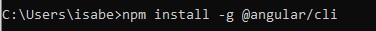
\includegraphics[scale=1]{npmangularcli}
\caption{Instalación de Angular CLI}
\end{figure}
Por último, desde la carpeta que ubica tanto el proyecto del museo (museo-eii) como el de la administración (museo-eii-admin), se ejecuta el comando \textit{npm install} para instalar los paquetes necesarios.
\begin{figure}[H]
\centering
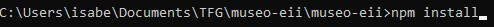
\includegraphics[scale=1]{npminstallmuseo}
\caption{Instalación de los paquetes del proyecto del museo}
\end{figure}
\begin{figure}[H]
\centering
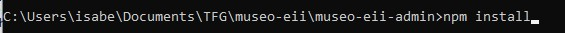
\includegraphics[scale=1]{npminstalladmin}
\caption{Instalación de los paquetes del proyecto de administración}
\end{figure}


\subsection{Manual de Ejecución} 
Las aplicaciones se encuentran desplegadas en un servidor Apache instalado en una máquina de la escuela:
\begin{itemize}
\item El museo en la dirección \url{http://156.35.163.193/museoeii.com}. 
\item La administración del museo en \url{http://156.35.163.193/museoeiiadmin.com}.
\end{itemize}
Para acceder a estas direcciones se debe estar conectado desde la  red de la Universidad de Oviedo, por lo que es necesario usar una VPN si queremos conectarnos desde una red externa, como se explica en \url{https://sic.uniovi.es/redes/accesoremoto}. 
\par Una vez completada la instalación siguiendo los pasos descritos en el apartado anterior, se pueden ejecutar ambas aplicaciones utilizando el comando \textit{ng serve -o}, \textit{npm start} o \textit{npm run ng serve -o}. Esto hará que la aplicación esté disponible en \url{http://localhost:4200}. Para ejecutarla de esta forma también es necesario estar conectado a la red de la Universidad, ya que la base de datos del sistema está alojada en la misma máquina que las aplicaciones desplegadas.
\begin{figure}[H]
\centering
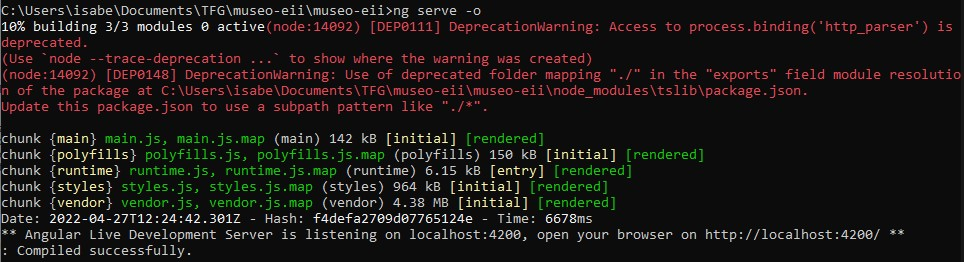
\includegraphics[scale=0.65]{ngservemuseo}
\caption{Ejecución de la aplicación del museo}
\end{figure}
\begin{figure}[H]
\centering
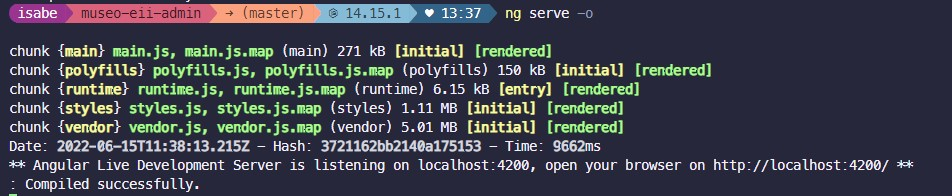
\includegraphics[scale=0.65]{ngserveadmin}
\caption{Ejecución de la aplicación de administración}
\end{figure}



\subsection{Manual de Usuario} 
\subsubsection{Museo}
Al acceder a la web observamos la página de inicio. La parte superior de esta página está presente en toda la aplicación web y, por orden de izquierda a derecha, observamos:
\begin{itemize}
	\item El logo de la escuela, que redirige a esta página de inicio.
	\item Museo, que redirige a la vista general del museo.
	\item Acerca de.
	\item Un selector de idioma, que permite cambiar entre inglés y español.
\end{itemize}
La parte inferior, que contiene enlaces a las redes sociales de la escuela, también está presente en toda la aplicación web.\par
En la parte central se encuentra el contenido específico de la página de inicio: una bienvenida a la página web y un botón que nos dirige a la vista general del museo.
\begin{figure}[H]
\centering
\centerline{
\includegraphics[scale=0.35]{homeIUDef}}
\caption{Manual de usuario: Inicio}
\end{figure}
En la vista general del museo hay una línea temporal y filtros de búsqueda.\par
En cada elemento de la línea temporal se muestra el nombre del periodo con un enlace al mismo, los años que comprende dicho periodo, y los nombres de los componentes pertenecientes al periodo, también con enlaces a cada uno de ellos.\par
La búsqueda puede realizarse por años o por nombre. Se puede filtrar por años mediante la barra deslizadora, y se mostrarán entonces todos aquellos periodos que, parcialmente o en su totalidad, tengan componentes pertenecientes a esos años. La búsqueda por nombre se realiza tras escribir en el recuadro de búsqueda y pulsar la tecla \textit{Enter}, y el resultado será aquellos periodos cuyo nombre o el nombre de alguno de sus componentes contenga el texto buscado.
\begin{figure}[H]
\centering
\centerline{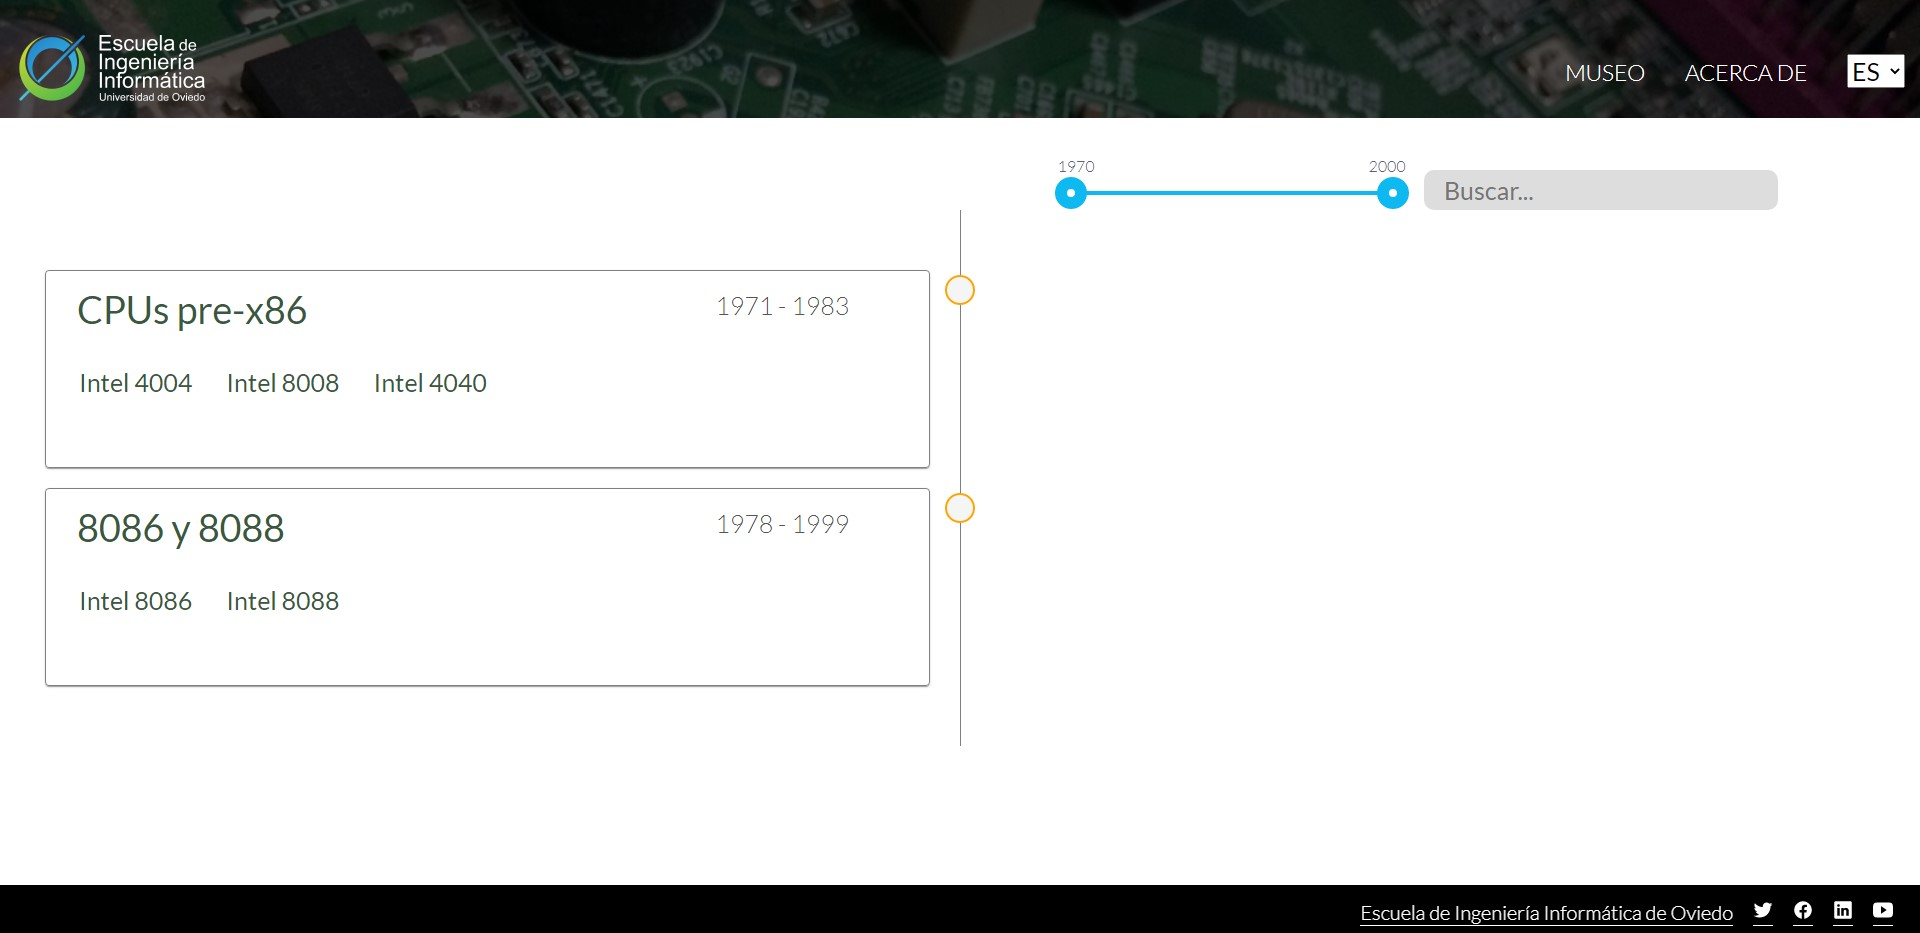
\includegraphics[scale=0.35]{museoIUDef}}
\caption{Manual de usuario: Vista general del museo}
\end{figure}
Al entrar en un periodo, en la parte superior podemos ver un menú, en la izquierda se mostraría el periodo anterior cronológicamente, y en la izquierda el periodo siguiente (si existen). El contenido principal de la página son los detalles del periodo: nombre, características, una lista de curiosidades (sabías que...), eventos informáticos ocurridos en esos años, los componentes pertenecientes al periodo (mostrando una imagen y el nombre, con un enlace al componente), y una serie de sistemas famosos que llevan esos componentes. 
\begin{figure}[H]
\centering
\centerline{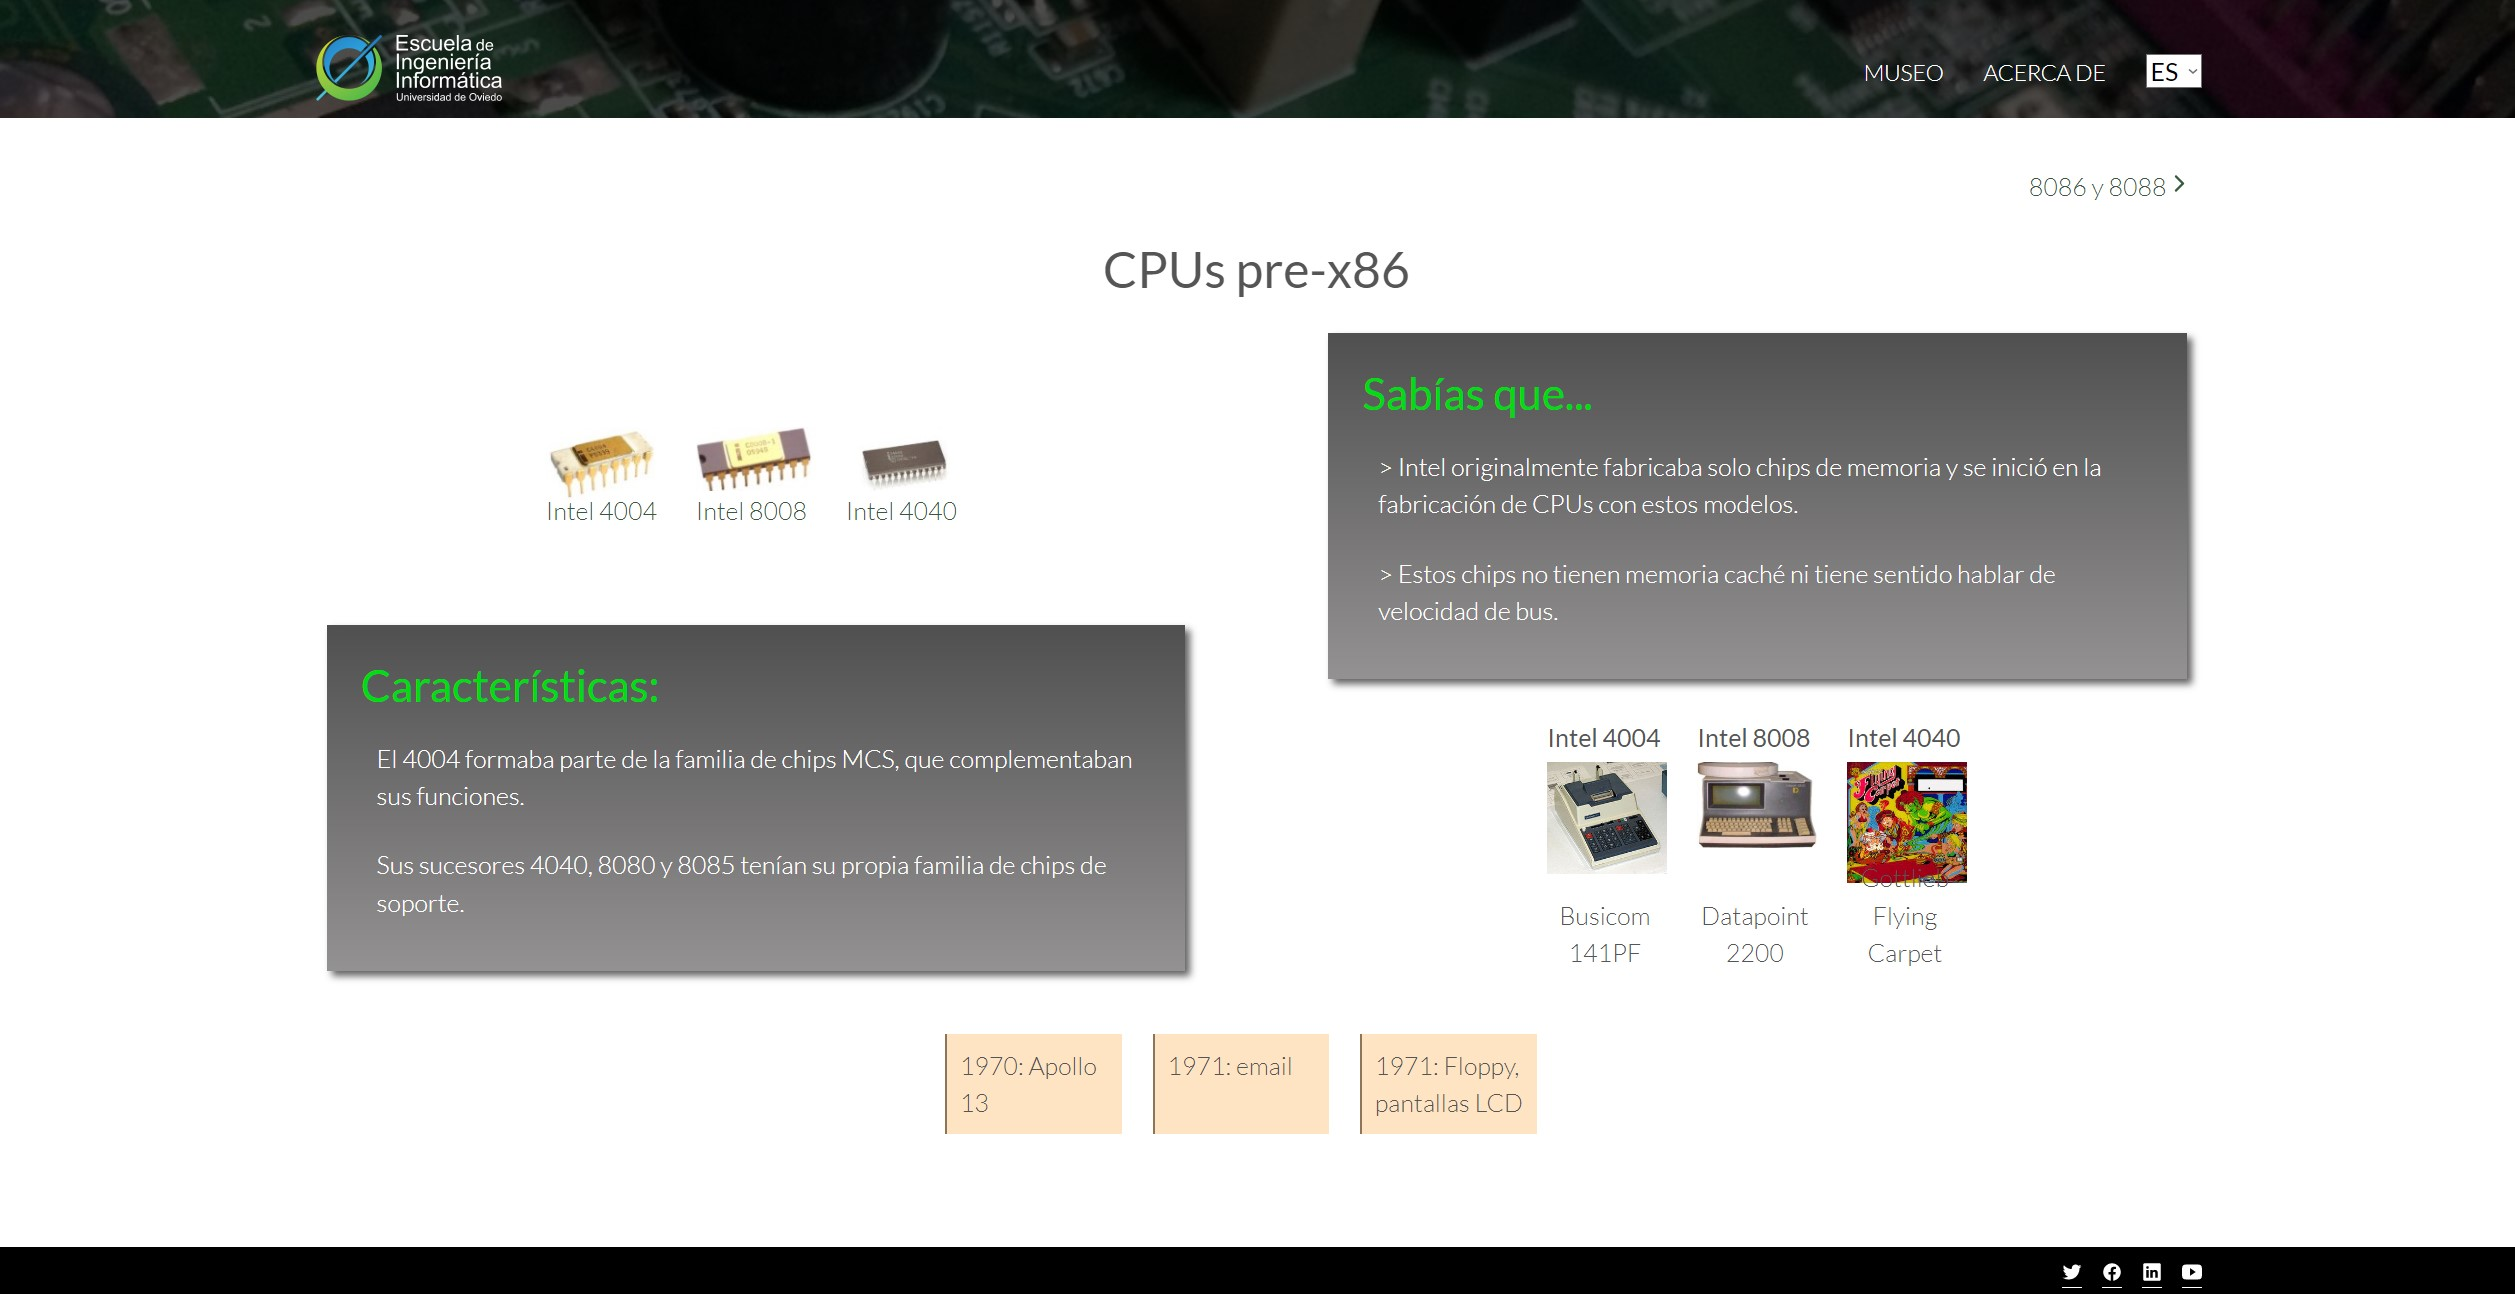
\includegraphics[scale=0.35]{periodoIUDef}}
\caption{Manual de usuario: Detalles del periodo (museo)}
\end{figure}
Por último, al acceder a un componente, podemos ver una galería de fotos que se abrirán en grande al pulsar sobre ellas, una descripción del componente y un listado de características. Además, en el lateral izquierdo hay un menú que permite navegar entre periodos (ver el anterior, el actual y el siguiente) y entre los componentes del periodo actual.
\begin{figure}[H]
\centering
\centerline{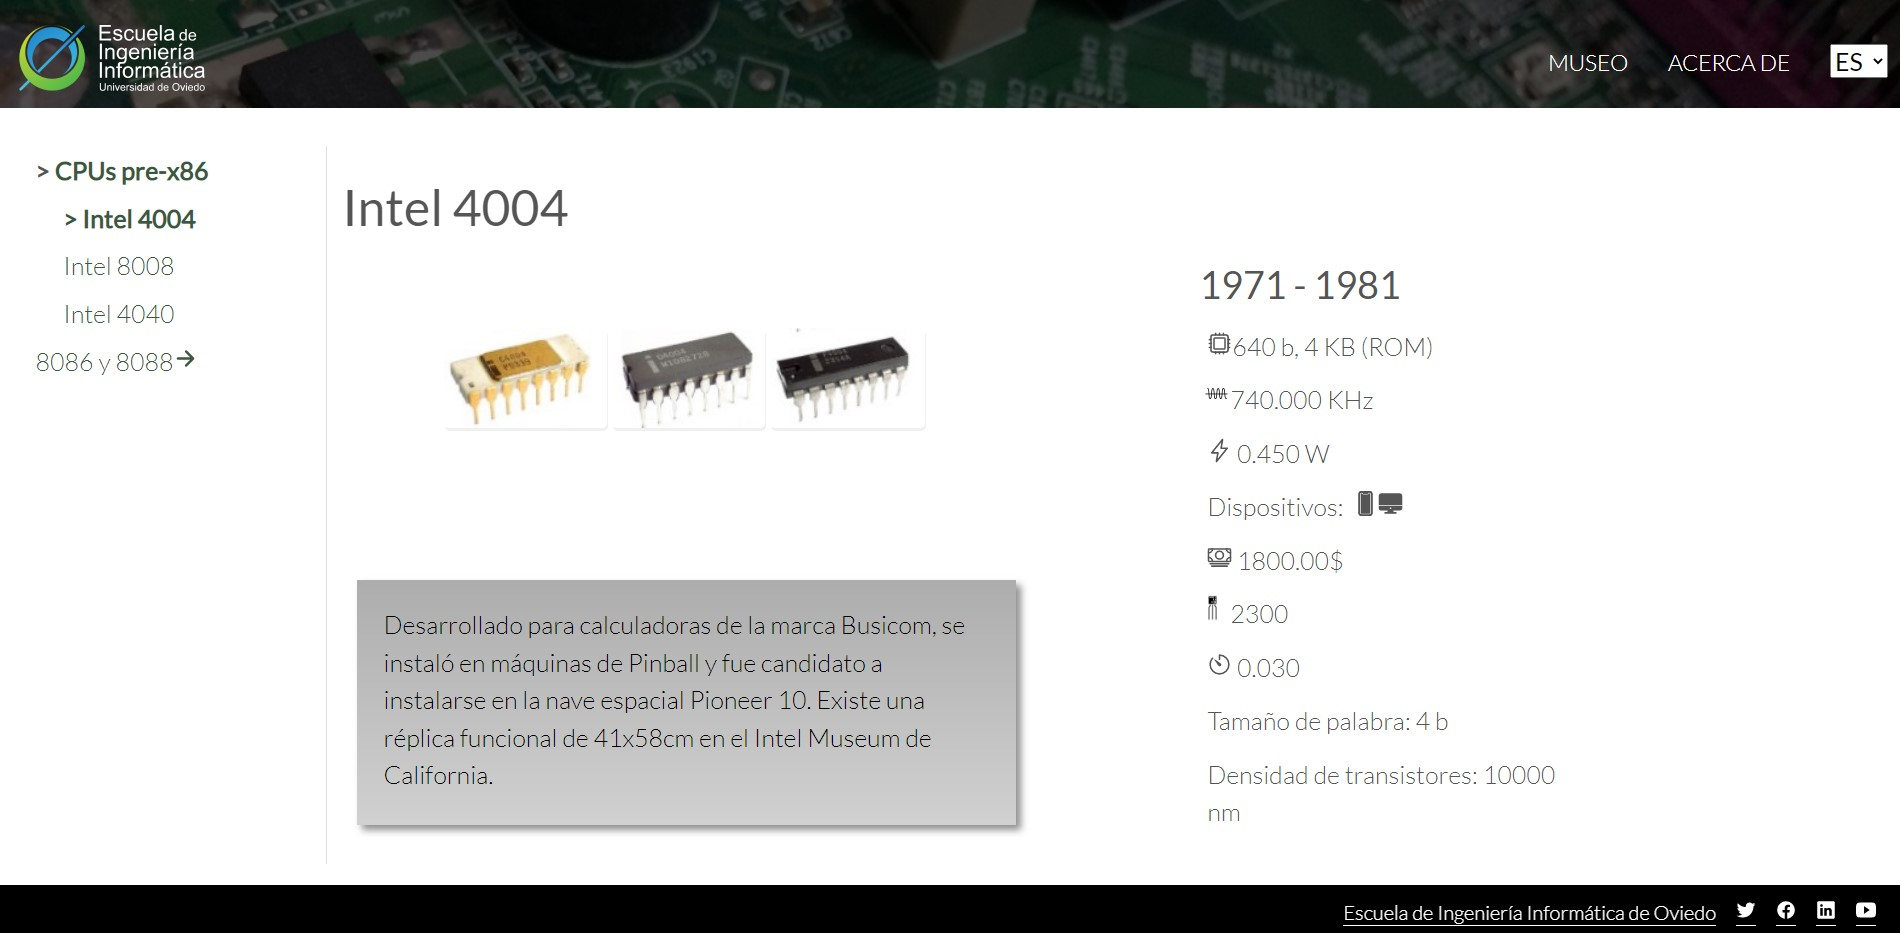
\includegraphics[scale=0.35]{piezaIUDef}}
\caption{Manual de usuario: Detalles del componente (museo)}
\end{figure}

\subsubsection{Administración del museo}
Al entrar a la web de administración del museo nos encontramos con el inicio de sesión. Es necesario indicar el correo electrónico y la contraseña para acceder.
\begin{figure}[H]
\centering
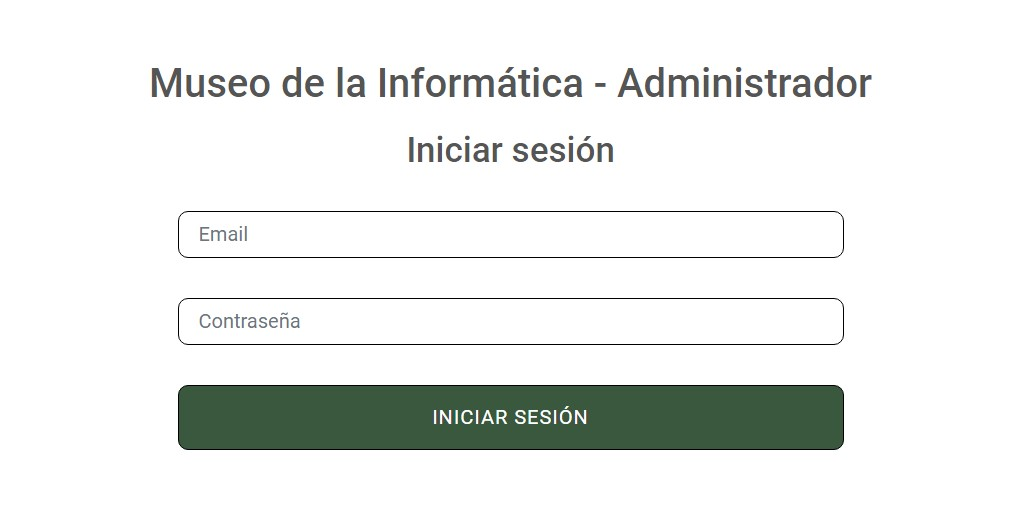
\includegraphics[scale=0.45]{loginIUDef}
\caption{Manual de usuario: Inicio de sesión}
\end{figure}
Si el administrador necesita cambiar la contraseña, podrá hacerlo accediendo a la máquina Ubuntu 20.04 donde se encuentra alojado el servidor Apache que contiene los archivos PHP y la base de datos del sistema, ya que habrá un fichero ejecutable que solicitará la nueva contraseña y realizará el cambio. Este fichero solo estará disponible en esta máquina ya que, al haber un solo usuario administrador, es más sencillo hacer el cambio de contraseña de esta forma en lugar de enviar un correo con un enlace temporal para realizarlo, y es seguro ya que el administrador es el único usuario con acceso a la máquina.
\begin{figure}[H]
\centering
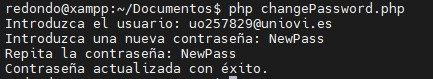
\includegraphics[scale=1]{changepassphp}
\caption{Manual de usuario: Cambio de contraseña}
\end{figure}
Lo primero que se muestra una vez iniciada la sesión es un listado de los periodos existentes, mostrando sus nombres con un enlace a cada uno de ellos, y permitiendo editar y eliminar cada periodo. Eliminar un periodo borrará también los componentes asociados al mismo, para ello se mostrará un aviso y se pedirá confirmación. En el lateral izquierdo hay un menú que se incluye en todas las páginas de la aplicación, desde el que se puede acceder a este listado de periodos, y a los formularios para añadir periodos y componentes.
\begin{figure}[H]
\centering

\includegraphics[scale=0.35]{listadoPeriodosIUDef}
\caption{Manual de usuario: Listado de periodos}
\end{figure}
Los detalles de un periodo y del componente muestran los mismos datos explicados anteriormente en el manual de usuario del museo, con la diferencia de en que cada una de estas páginas se muestra una opción para editar el periodo o el componente que estemos visualizando, y en el listado de componentes del periodo también se da la opción de editar o eliminar cada uno de ellos.
\begin{figure}[H]
\centering
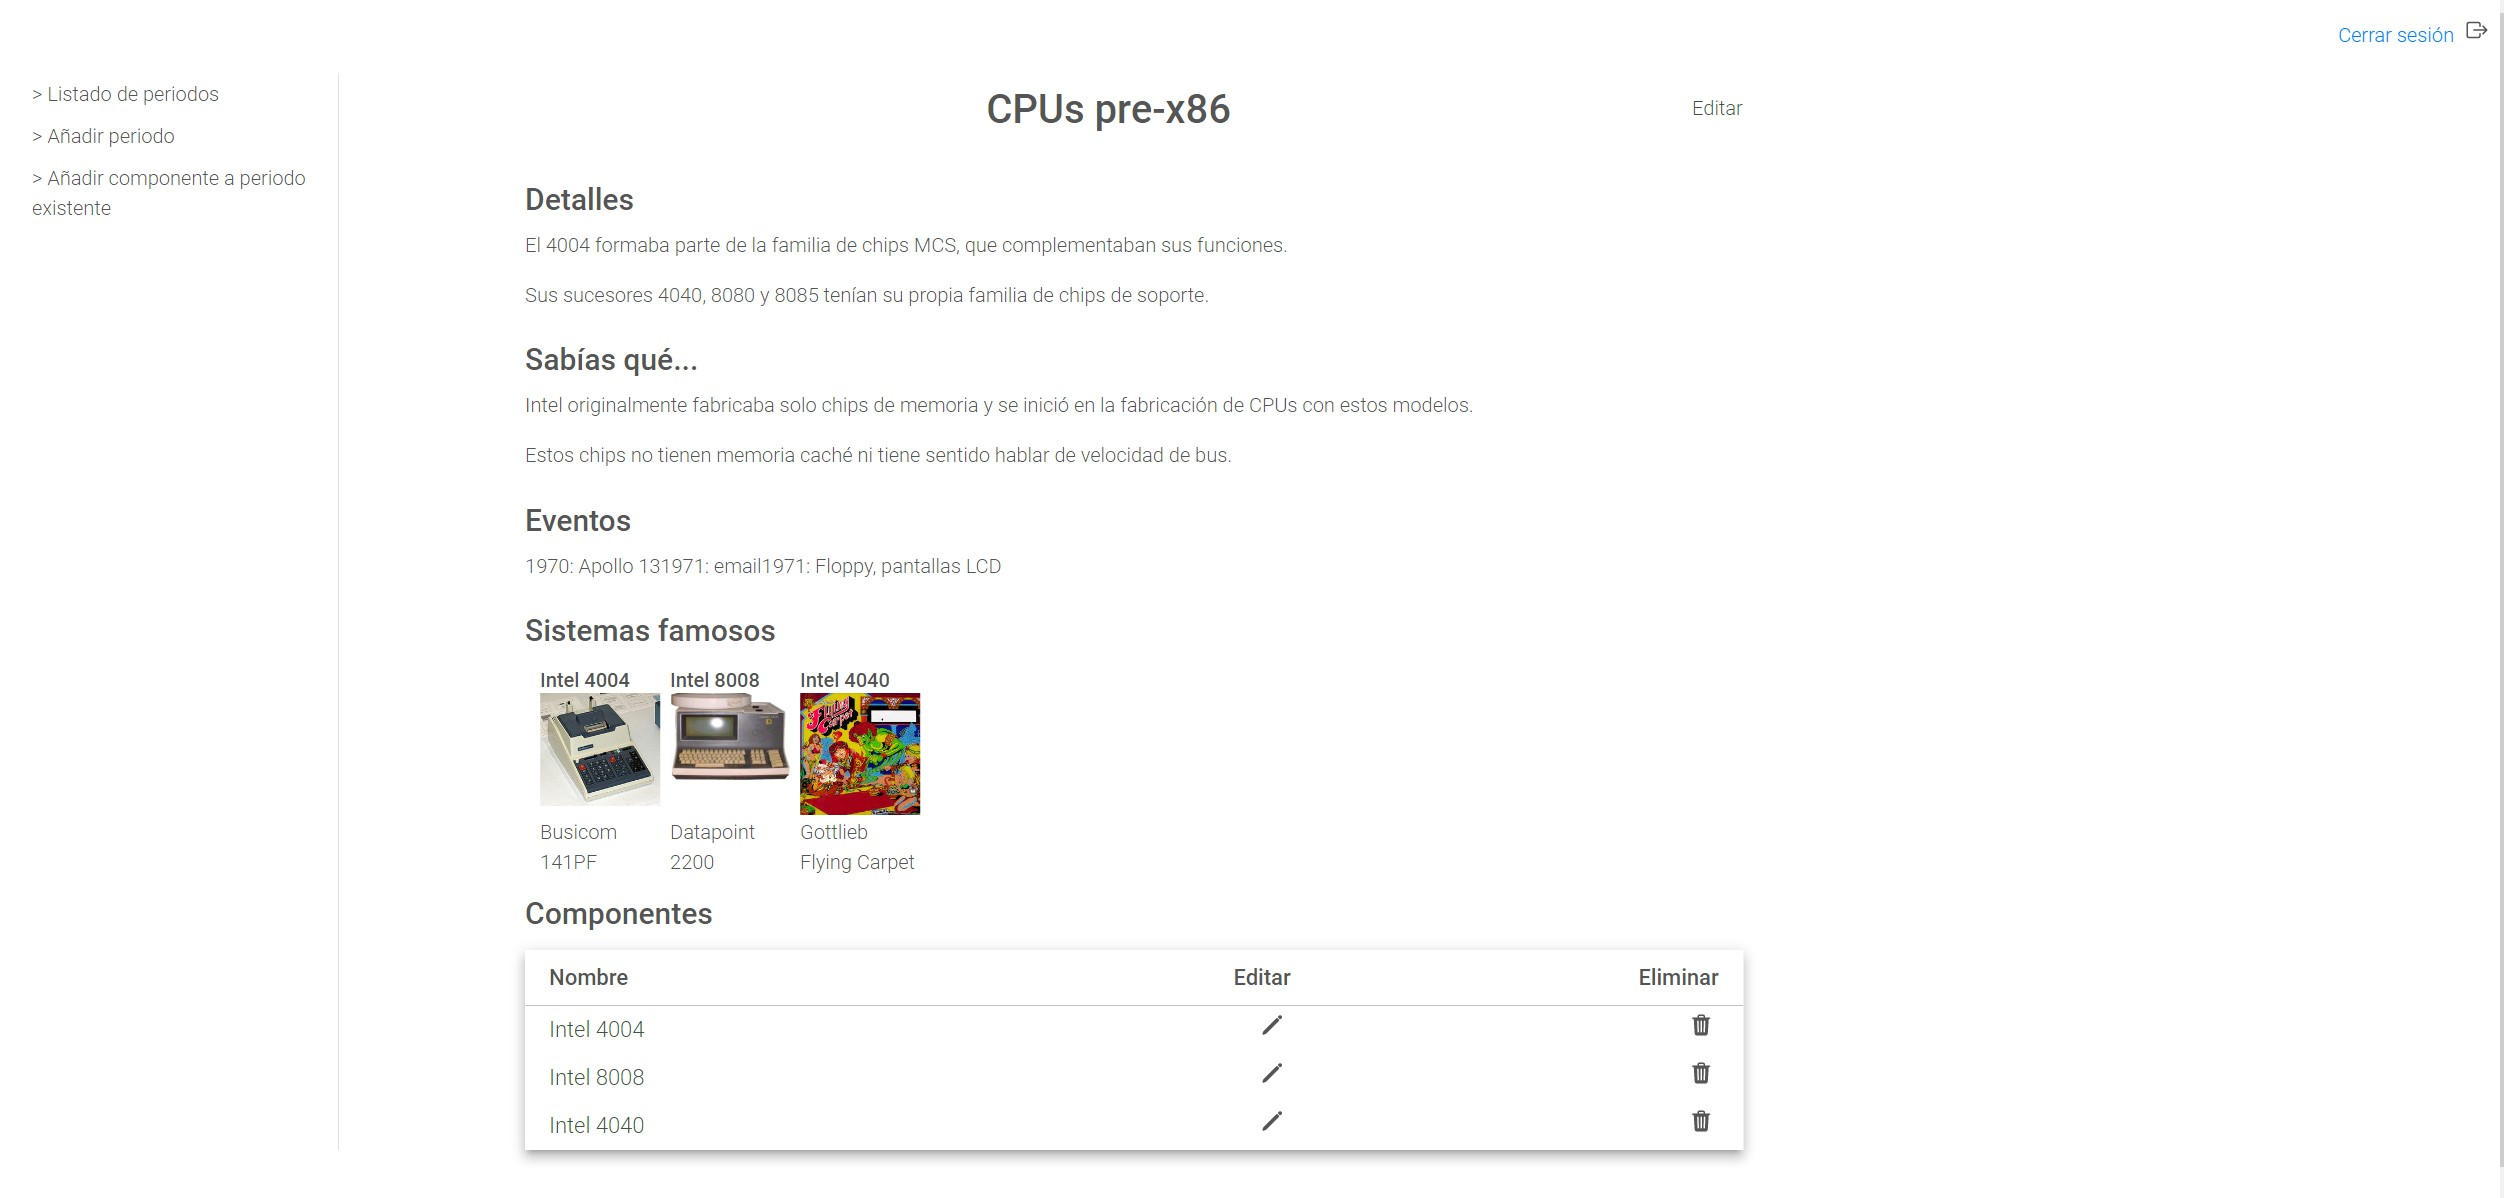
\includegraphics[scale=0.35]{periodoIU2Def}
\caption{Manual de usuario: Detalles de un periodo (administración)}
\end{figure}
\begin{figure}[H]
\centering
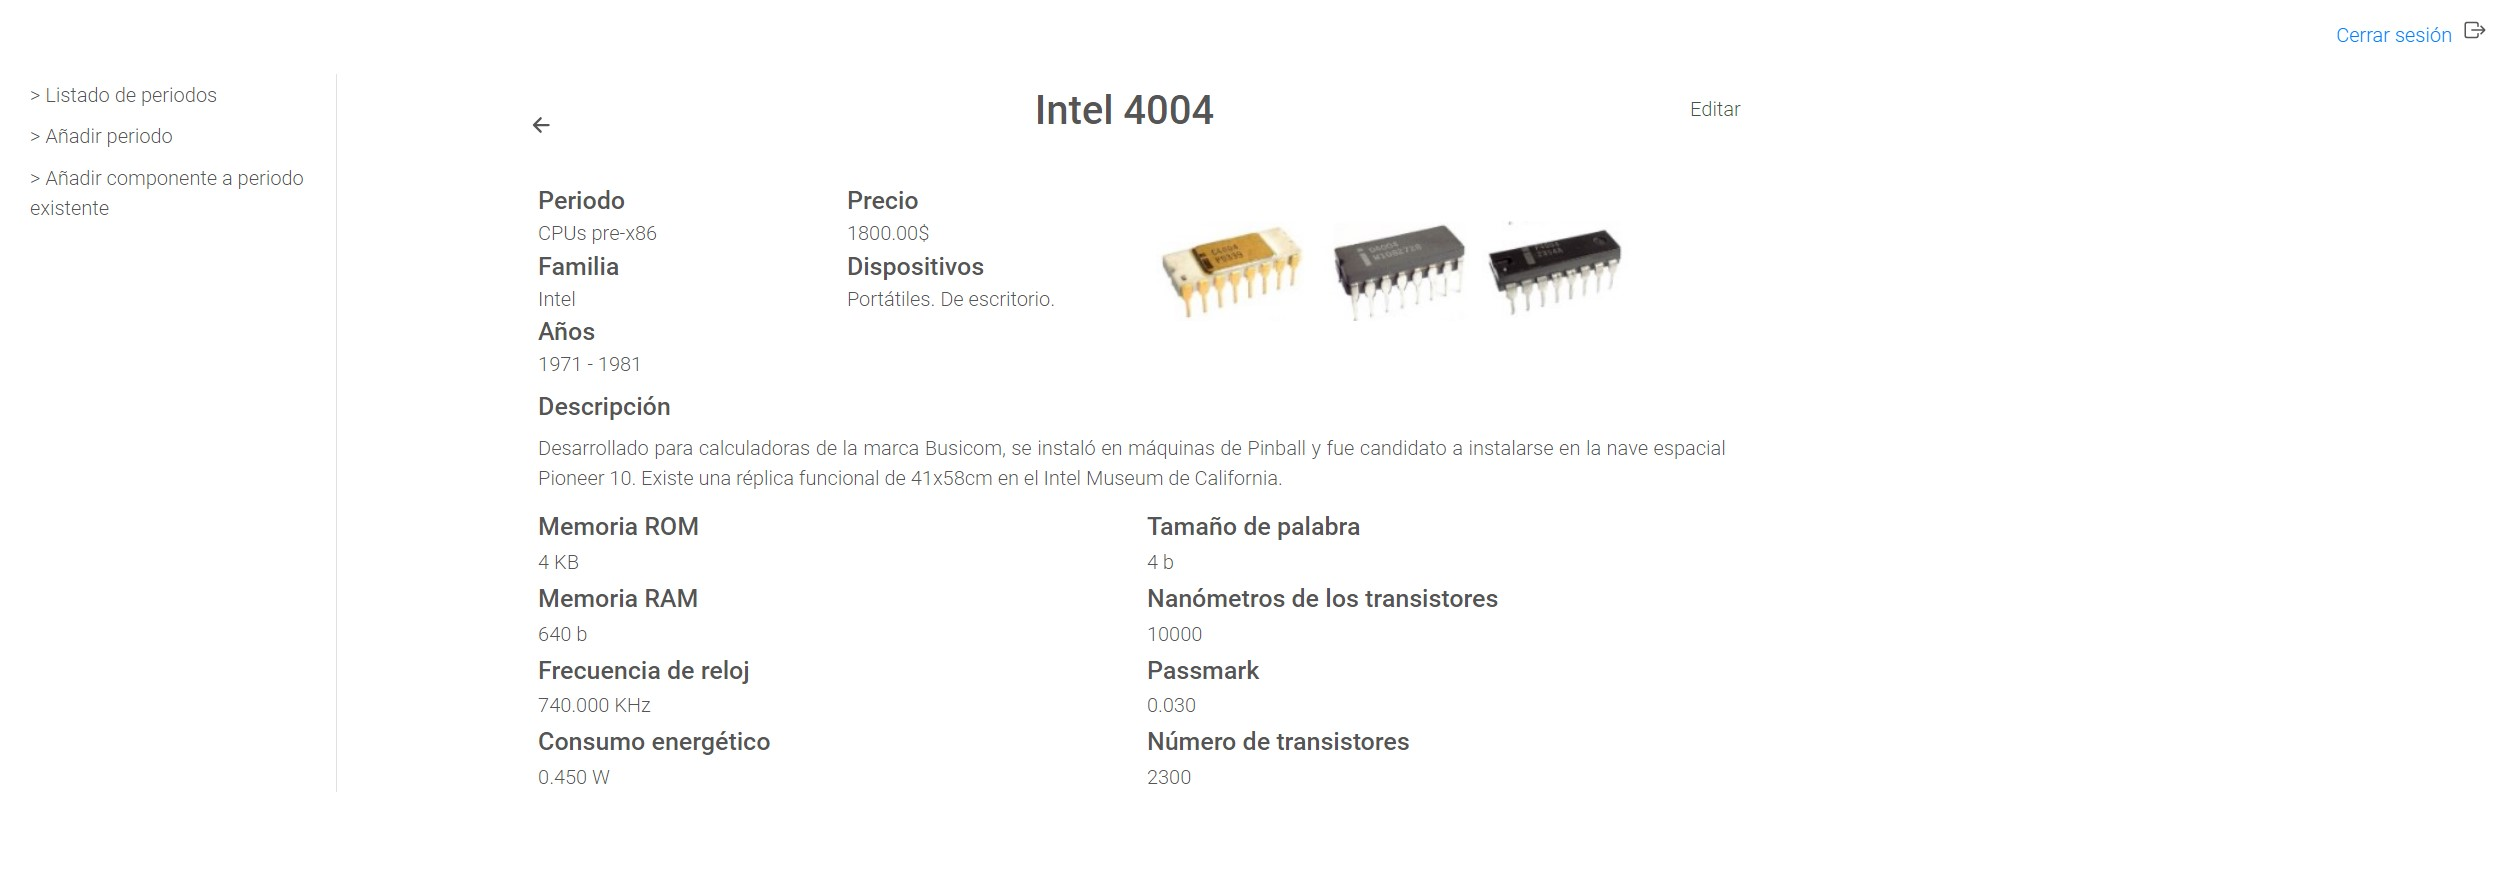
\includegraphics[scale=0.35]{compIUDef}
\caption{Manual de usuario: Detalles de un componente (administración)}
\end{figure}
En el formulario de añadir un periodo hay cuatro entradas de texto para nombre, detalles, curiosidades y eventos del periodo. Todos ellos deben rellenarse obligatoriamente para poder guardar el periodo. Si se pulsa el botón \textit{Cancelar}, el formulario se vaciará de nuevo. Al pulsar \textit{Guardar y continuar} con el formulario completo, se añadirá el periodo a la base de datos del sistema y nos redigirá al formulario para añadir componentes. En cambio, si el formulario no es válido se mostrará un error y no se añadirá.
\begin{figure}[H]
\centering
\includegraphics[scale=0.35]{añadirPeriodoIUDef}
\caption{Manual de usuario: Formulario para añadir un periodo}
\end{figure}
A la hora de editar un periodo, el formulario funcionará igual que al añadirlo, con la diferencia de que los valores iniciales serán los del periodo que se está editando.
\begin{figure}[H]
\centering
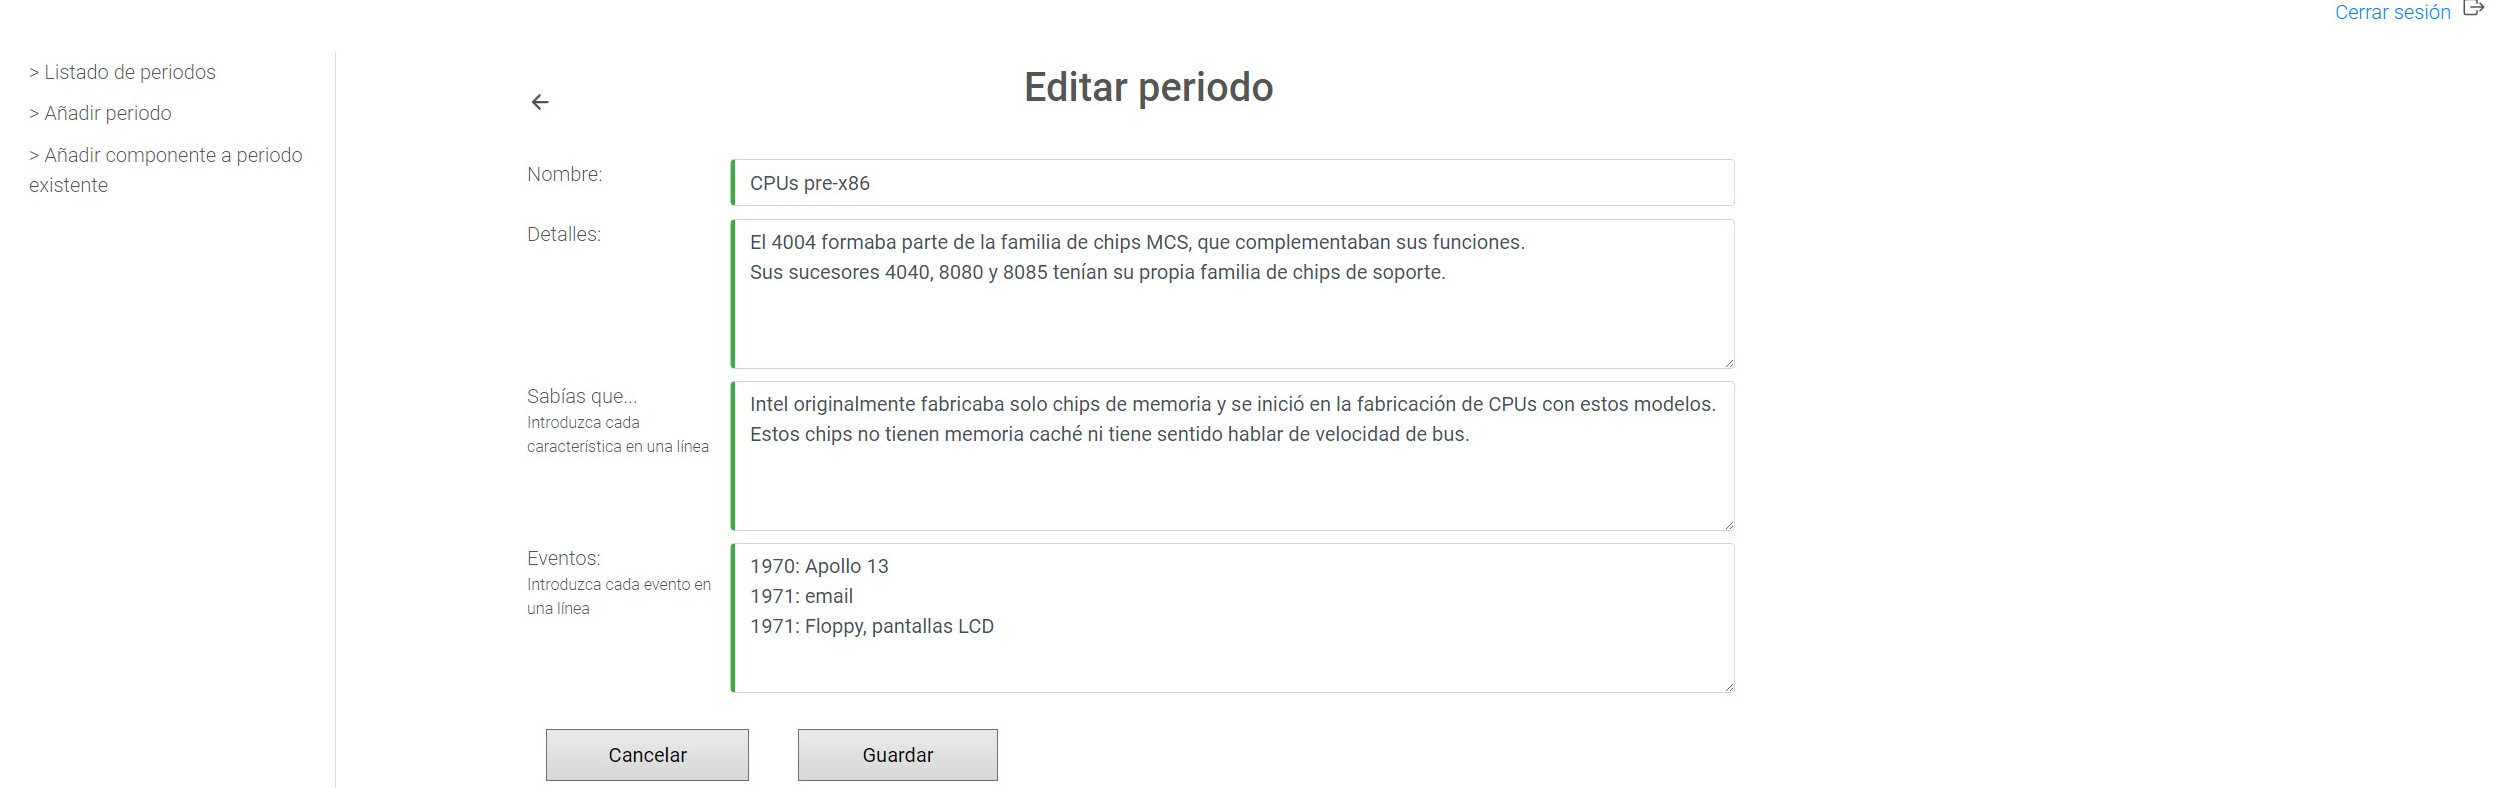
\includegraphics[scale=0.35]{editarPeriodoIUDef}
\caption{Manual de usuario: Formulario para editar un periodo}
\end{figure}
Los formularios para añadir y editar componentes funcionan de la misma forma que los de añadir y editar periodos, pero en este caso, hay campos que no son obligatorios, como la subida de imágenes y el sistema famoso. Además, al añadir o editar componentes se puede seleccionar su tipo: CPU o componente genérico. Al seleccionar CPU se muestran los campos de memoria ROM, memoria RAM, frecuencia de reloj, consumo energético, tamaño de palabra, nanómetros de transistores, passmark y número de transistores.
\begin{figure}[H]
\centering
\includegraphics[scale=0.35]{añadirCompIUDef}
\caption{Manual de usuario: Formulario para añadir un componente}
\end{figure}
\begin{figure}[H]
\centering
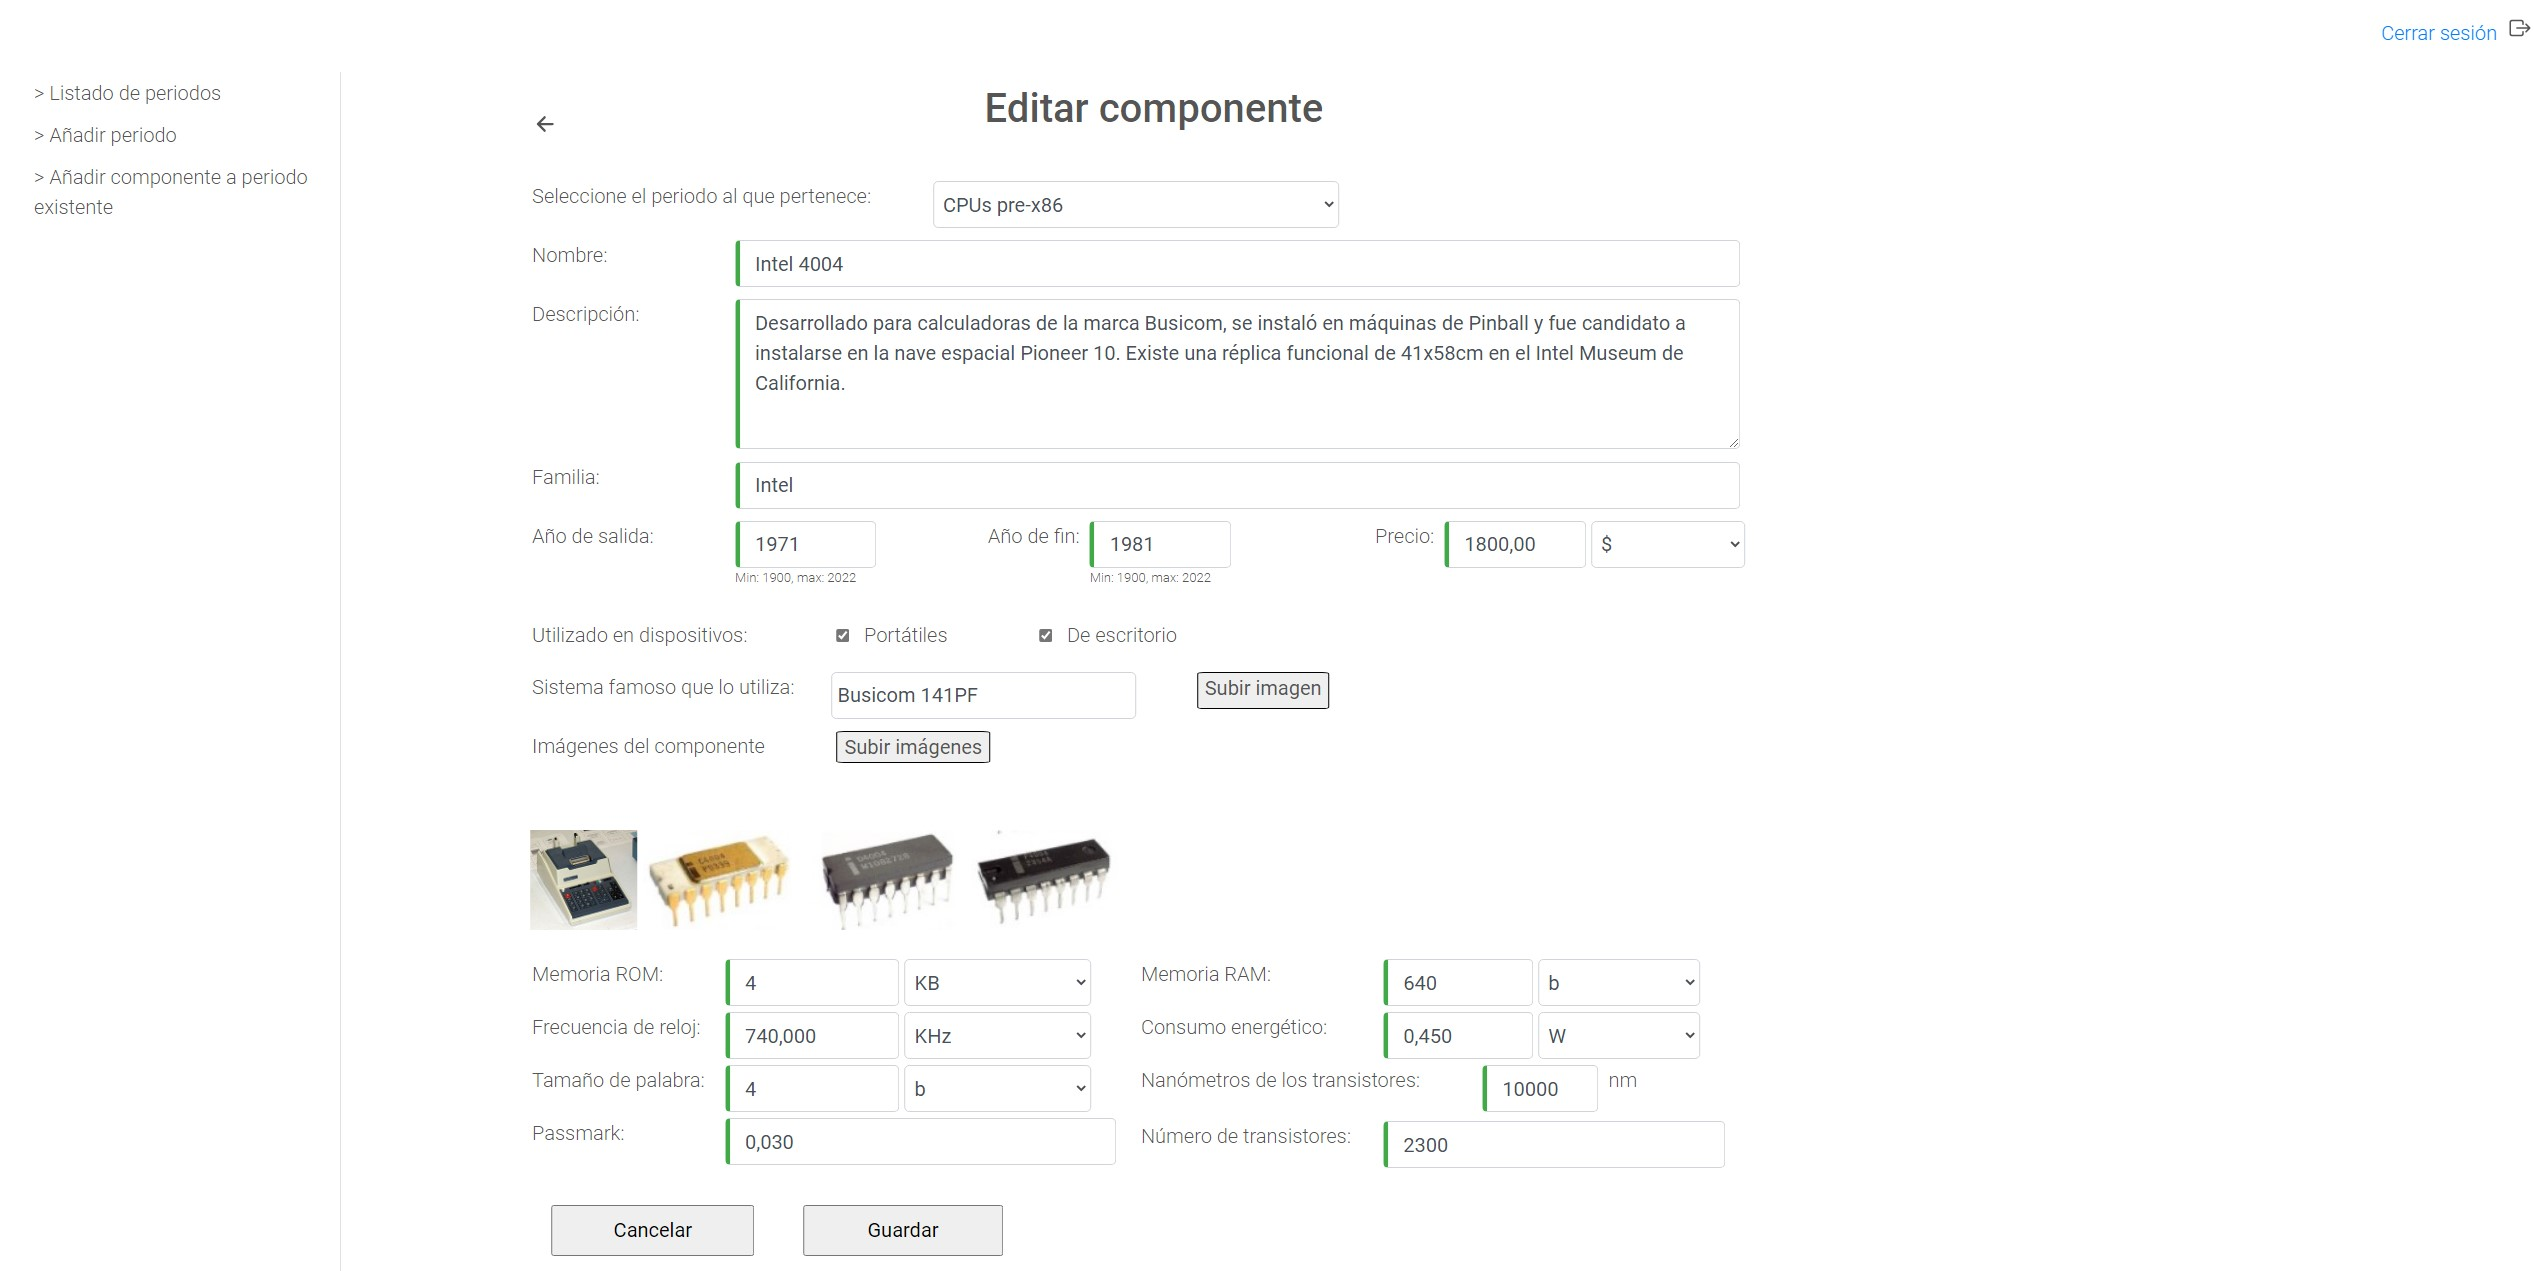
\includegraphics[scale=0.35]{editarCompIUDef}
\caption{Manual de usuario: Formulario para editar un componente}
\end{figure}


\subsection{Manual del Programador}
En este manual se explicará cómo ampliar la aplicación añadiendo nuevos tipos de componentes además de CPUs. Primero habría que crear una nueva clase para cada tipo que se desee añadir. Cada una de estas clases implementarán la interfaz \textit{MyComponent} y heredarán de \textit{GenericComp}. También habría que actualizar la enumeración \textit{CompTypes}. Estos tres elementos mencionados se encuentran en el archivo \textit{comp.ts}, que forma parte tanto del proyecto del museo (museo-eii) como de la administración (museo-eii-admin). Una vez realizado esto, común a ambos proyectos, se explicará qué debe añadirse a cada uno de ellos en específico, así como a la base de datos.

\subsubsection{Museo}
En el proyecto del museo (museo-eii) deberá generarse un componente de Angular para cada tipo añadido, se llamará \textit{`new type`DetailsComponent} y será hijo de \textit{CompDetailsComponent}, del que recibirá como input el atributo \textit{comp}. Este solo se mostrará cuando \textit{comp} sea una instancia del tipo correspondiente a `new type`. En \textit{`new type`-details.component.html} se listarán las características de \textit{comp}.\par
Además, en el método \textit{getComp} de \textit{CompDetailsComponent} habrá que añadir las comprobaciones necesarias para mostrar los nuevos tipos definidos.

\subsubsection{Administración del museo}
En el proyecto de la administración (museo-eii-admin) habrá que generar dos componentes de Angular nuevos por cada tipo añadido: 
\begin{itemize}
\item \textit{`new type`FormComponent}, hijo de \textit{AddCompComponent} y de \textit{EditCompComponent}. De ambos recibe como input el atributo \textit{model}. En \textit{`new type`-form.component.html} se incluirán los campos del formulario que se correspondan con las características del tipo creado. Se mostrará cuando \textit{model} sea una instancia del tipo correspondiente a `new type`. \par
En el método \textit{createModel} de \textit{AddCompComponent} habrá que añadir la opción de crear un objeto de este nuevo tipo, y también se añadirán las comprobaciones necesarias en los métodos \textit{isValid} y \textit{cloneComp} de \textit{AddCompComponent} y \textit{EditCompComponent}.
\item \textit{`new type`DetailsComponent}, hijo de \textit{MyComponentComponent}, del que recibe como input el atributo \textit{c}. En este caso, se hará exactamente lo mismo que lo mencionado anteriormente al añadir \textit{`new type`DetailsComponent} en el proyecto del museo, ya que ambos componentes son para mostrar las características de cada tipo.
\end{itemize}

\subsubsection{Base de datos}
En la base de datos habría que crear una tabla por cada nuevo tipo de componente, con los campos necesarios para este que no estén ya incluidos en la tabla \textit{components}. La clave primaria de esta tabla sería también una clave foránea, el identificador del componente en la tabla \textit{components}. Una vez creadas las tablas correspondientes, habría que modificar las comprobaciones y consultas realizadas en los archivos \textit{getComp.php, updateComp.php} y \textit{postComp.php} para incluir los nuevos tipos creados.


%\newpage
%\section{CSI 8: CONSTRUCCIÓN DE LOS COMPONENTES Y PROCEDIMIENTOS DE MIGRACIÓN Y CARGA INICIAL DE DATOS}


